\chapter{State of the art}

\label{sec:state-of-art}

    This chapter aims to provide a literature overview of the topics that relate to the main problem that this thesis aims to help solve, which is the lack of cooperation between applications and the service providers of the infrastructure where such applications reside.
    As such, focus is given on discussing structural network patterns utilized by applications to give them particular properties which are helpful to achieve their use case.
    Among these patterns, particular interest will be given to three of them for the following reasons: firstly, due to their popularity in the current network paradigm; secondly, due to their potential to optimize traffic that is generated at the application level.
    Considering this, the patterns that will be discussed are the distributed approach of \gls{p2p} architectures on Section \ref{sec:state-p2p}, the quite recently popular \glspl{cdn} on Section \ref{sec:state-cdn}, and the classic client-server model on Section \ref{sec:state-client-server}.
    For each of these, a conceptual analysis is made - more specifically, contextual background, the architecture itself, advantages and disadvantages, and possible use cases.
    Additionally, there's an examination on how applications that utilize these patterns affect, positively or negatively, the physical infrastructure where they operate on, and where does potential reside for mutually-beneficial cooperative behaviour between these two layers.
    Following this, Section \ref{sec:state-solutions} displays existing proposals for increased layer cooperation, and alongside it a discussion on the practical consequences of adopting them.
    Finally, Section \ref{sec:state-alto} gives special attention to the \gls{alto} working group's proposal for a layer-cooperative system, as it is the baseline for this thesis's work.

\section{Peer-to-Peer (P2P) Networks}

\label{sec:state-p2p}

\subsection{Concepts and Applications}

    Due to the many hybrid implementations that have surfaced, the definition of a \gls{p2p} network has become harder to pinpoint.
    Nevertheless, a \gls{p2p} network is grounded on some properties, among them that it consists of many singular computing elements, the "peers", which have between themselves similar privileges and functions (this contrasts with the client-server architecture, where two different roles exist - the one that provides a service and the one that can consume it - with functionality and control being thus centralized).
    \gls{p2p} networks decentralize computational resources as a means to achieve a given task in a way that is inherently different from a centralized counterpart.
    This decentralized architecture of the entire system as a whole gives it an interesting list of properties, among them:

\begin{itemize}
    \item \textbf{Dynamic scaling}: As all member nodes can share their computing resources with the network, the system increases its capacity with an increase in its users.
        As a new peer acts as client to the network, scaling the service becomes less of a challenge as each new client will also act as a server.
        This then removes the necessity to manage how many service resources are needed - the amount of existing resources is linked to the number of existing clients, and thus there's no need to purchase and manage central resources, as the network dynamically allocates them by nature.
    \item \textbf{Resilience to failure}: Whereas centralized solutions are much more vulnerable to node and link failures, a decentralized one can more easily work around such threats - as all peers can encompass the same server functionality, network services and resources are not provided on a limited set on nodes, but instead can be redundantly deployed throughout as needed.
    \item \textbf{Power decentralization}: As a consequence to sharing server roles and resources, no single peer has direct control of the network, and the information is not centralized.
        As such, this considerably deters any attempts to overpower the network, e.g., via means of censorship or biased node favoring.
\end{itemize}

    These, however, are not without their nuances - since many \gls{p2p} hybrids exist, these properties are not immutable.
    For example, if we consider BitTorrent, which has tracker servers to redirect users to a correct peer with the requested resource, whilst the network itself can still be resilient to failure, the content-retrieval service that the \gls{p2p} network provides has a single point of failure and of control - the trackers themselves.
    Furthermore, the \gls{p2p} network design brings, by its nature, alongside their potentially advantageous properties, also some some potentially disadvantageous ones to consider:

\begin{itemize}
    \item \textbf{Security hazards:} The equal functionality property that \gls{p2p} networks have give peers much power to influence others.
        Without proper care, malicious peers are a security risk.
    \item \textbf{Management:} Since resources and services are not centralized, tasks such as event logging and resource backups become very difficult, and perhaps impossible if the peers do not abide by any proper orchestration strategies.
\end{itemize}

    \gls{p2p} applications have had, in the past decades, a mainstream image that is plagued with legality and security issues.
    Nonetheless, its design possesses many interesting properties - some of them displayed above - that make it fitting for varied use cases, e.g., file sharing, media streaming, social networking, and computation with distributed and cooperative algorithms.

    Despite their reputation, the influence of \gls{p2p} applications is undeniable: Sandvine \cite{sandvine} published a global Internet phenomena report concluding that BitTorrent alone had, in 2019, a global application total traffic share of 2.4\%, but perhaps most importantly over 27\% of total upstream volume of traffic, with that value being 44\% for \gls{emea} alone \cite{sandvine2019}.

    Beyond file sharing purposes, \gls{p2p} applications have been recently considered a fitting solution for low-cost content delivery systems in high demand scenarios - for example, in applications such as PPStream \cite{ppstream} in China, which provide television content over IP to large audiences.
    Similarly, Akamai \cite{akamai} recognizes the potential of \gls{p2p} technologies to provide a highly distributed option for serving static content over the network, although it being currently lacking in management and control features \cite{akamai-report}.
    Indeed, \gls{p2p} Internet video broadcast services - and world-wide static content delivery services for that matter - seem attractive as they are cost-effective and easy to deploy, and are fitting for large scale demands, and thus have the potential to become a more mainstream solution \cite{jiangchuanliu2008}.

    Concluding, the \gls{p2p} network architecture has many appropriate use cases, and their rather different strategy, compared to the client-server architecture, gives it many potentially interesting properties for users and \glspl{isp}.
    Considering its large global traffic share, particularly in upstream traffic, and its potential adoption towards the large scale demands of the future, \gls{p2p} applications are likely to persist and will be in the minds of \gls{isp} administrators for the near future.

\subsection{Architecture}

    As stated previously, the term "Peer-to-peer" has become very broad and now serves as an umbrella for many different variations of the core decentralized architecture design.
    Thus, this section focuses not on giving an overview of a single conceptual architecture of what defines a \gls{p2p} network, but instead of the many existing variations and how they differ among themselves.
    All \gls{p2p} networks are characterized by consisting of peers that know one another as to form a so-called overlay network on top of its supporting underlay network.
    How peers are organized in these \gls{p2p} networks and how they operate is what distinguishes the many sub-types.
    Table \ref{table:p2p-structures} groups known \gls{p2p} systems in regards to their centralization and structure, similar to the groupings of \cite{p2p-survey-1} and \cite{p2p-survey-2}, with the latter further distinguishing the protocols in regards to other parameters, e.g., security, reliability, and performance.
    The rest of this section follows the survey made by the former.

    One would expect that all \gls{p2p} applications would have no centralization at all, since the \gls{p2p} design ponders functionality spread throughout the network.
    However, some modifications have been made in some of these sub-types, which shift how much decentralization they really have in practice.
    Similarly, different strategies exist that dictate the structural hierarchy that resides within the member peers.
    As would be expected, these sub-types of \gls{p2p} networks thus possess different strengths and weaknesses, and these can be leveraged to the most appropriate use cases.

\begin{table}[h]
\caption{Types of P2P systems (Adapted from \cite{p2p-survey-1})}
\label{table:p2p-structures}
\begin{adjustbox}{max width =1.1\textwidth,center}
\begin{tabular}{lllllll}
                                                 &                                        &                                                                                 &                                                                                                                 &                                                                                                                          &  &  \\ \cline{3-5}
                                                 & \multicolumn{1}{l|}{}                  & \multicolumn{3}{c|}{\textbf{Centralization}}                                                                                                                                                                                                                                                                                          &  &  \\ \cline{3-5}
                                                 & \multicolumn{1}{l|}{}                  & \multicolumn{1}{l|}{Hybrid}                                                     & \multicolumn{1}{l|}{Partial}                                                                                    & \multicolumn{1}{l|}{None}                                                                                                &  &  \\ \cline{1-5}
    \multicolumn{1}{|c|}{\multirow{9}{*}{\textbf{Structure}}} & \multicolumn{1}{l|}{None}              & \multicolumn{1}{l|}{\begin{tabular}[c]{@{}l@{}}BitTorrent, Napster,\\ Publius\end{tabular}} & \multicolumn{1}{l|}{\begin{tabular}[c]{@{}l@{}}Kazaa,\\ Morpheus,\\ Gnutella (extension proposals),\\ Edutella\end{tabular}} & \multicolumn{1}{l|}{\begin{tabular}[c]{@{}l@{}}Gnutella,\\ FreeHaven\end{tabular}}                            &  &  \\ \cline{2-5}
\multicolumn{1}{|c|}{}                           & \multicolumn{1}{l|}{In Infrastructure} & \multicolumn{1}{l|}{}                                                           & \multicolumn{1}{l|}{}                                                                                           & \multicolumn{1}{l|}{\begin{tabular}[c]{@{}l@{}}Chord,\\ CAN,\\ Tapestry,\\ Pastry\end{tabular}}                          &  &  \\ \cline{2-5}
\multicolumn{1}{|c|}{}                           & \multicolumn{1}{l|}{In System}         & \multicolumn{1}{l|}{}                                                           & \multicolumn{1}{l|}{}                                                                                           & \multicolumn{1}{l|}{\begin{tabular}[c]{@{}l@{}}BitTorrent (DHT/Trackerless), \\OceanStore,\\ Mnemosyne,\\ Scan, \\ PAST,\\ Kademlia,\\ Tarzan\end{tabular}} &  &  \\ \cline{1-5}
                                                 &                                        &                                                                                 &                                                                                                                 &                                                                                                                          &  &
\end{tabular}
\end{adjustbox}
\end{table}

    Early versions of Gnutella \cite{gnutella} come as a famous example of a decentralized and unstructured architecture, as peers act with equal functions and privileges, and no inherent structure exists for peers to connect to each other, nor does it for storing or retrieving content on the overlay network.
    The bootstrapping phase consists of users reading from list containing a set of Gnutella peers - a list that is retrieved from a trustworthy source - and attempting to connect to each one of them until a preferred number of known neighbours is reached.
    The unstructured nature of this protocol makes it so there's no systematic way to efficiently retrieve content, and thus a technique of flooding the network with content queries is used until either a reply is met or the predefined TTL value is exceeded, as is exemplified in Figure \ref{fig:gnutella-flood}.

\begin{figure}[!h]
\centering
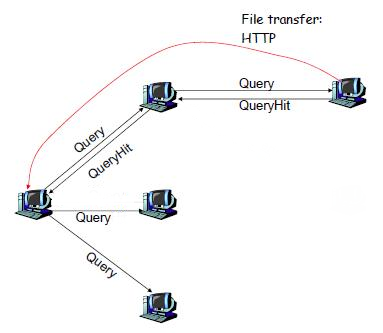
\includegraphics[scale=1.5]{img/gnutella-flood.png}
\caption{Demonstration of Gnutella's file searching mechanism \cite{gnutella-flood}}
\label{fig:gnutella-flood}
\end{figure}

    Partially centralized architectures were defined as similar to those which are decentralized, but with the added caveat that some peers are chosen to service a portion of the network.
    This is done to take use from the fact that not all network peers are alike in terms of memory, computational power, or other relevant resources.
    As such, more capable peers are elected as "super nodes" and are delegated with more responsibilities, noting that the network self-configures in situations where such elected nodes either fail or willingly leave the network, and as such there is no single point of failure as there would be on a true centralized architecture.

    A hybrid architecture approach in a \gls{p2p} network employs some elements from the client-server architecture.
    With Napster \cite{napster} as an example, whilst peers still operate as servers or clients, they must contact an intermediary and central server when querying for content, which will in turn redirect them to one or many peers that contain it - a similar concept applies for BitTorrent, where such intermediary servers are called trackers.
    Obviously, the choice to add a centralized aspect to the architecture hinders many of the advantages from a purely unstructured solution - namely its scalability, resilience to failure, and decentralization of control - serving as a trade-off to facilitate the control and maintenance of the network, as well as the peers' ability to bootstrap to it and locate content.

    A \gls{p2p} architecture is structured if it employs some non-random and systematic criteria on how the network operates, e.g., how peers organize themselves and where content is stored and how it it retrieved.
    For example, FreeNet \cite{freenet} uses the content's hash as a key that is used to query for it, and which in turn is used by the peers in each subsequent hop to know where to forward the request, instead of flooding the network in attempts to blindly find it like Gnutella does.
    Many of the structured \gls{p2p} architectures rely on \glspl{dht}, which act as a decentralized map structure that binds a given key to some content in the network, in such a way that the full key-space is partitioned over the peers.
    Two examples of structured \gls{p2p} architectures that use \glspl{dht} can be seen in Figure \ref{fig:dht-usage}. Specifically, Figure \ref{fig:chord} displays how the Chord algorithm uses a circular \gls{dht} where each peer knows the location of some peers that are their predecessors, and some that are their successors.
    When a peer needs to query for some content, it uses its key to firstly search for it locally and, if it doesn't exist, it forwards the query to their successors, and the process recursively continues.
    On the other hand, Figure \ref{fig:can} display how \gls{can} has the key-space mapped to a virtual two dimensional grid, and its area is partitioned to peers considering a deterministic function, which in turn is used by querying peers to figure out where a given content is stored.
    A straight arrow from querying node to providing node represents the routing path that the querying message must travel: A-B-E.

    Employing a systematic way to self-organize and share content is the means to guarantee that a \gls{p2p} network can be fully decentralized whilst maintaining a desirable level of performance.
    However, the reliance on structure means that it must be maintained, e.g., managing neighbour pointers on Chord or managing area allocations on CAN, and that can be costly or even impossible with high rates of peer churn, i.e., with a sufficiently large rate of peers entering and leaving the network.

\begin{figure}[t!h]
    \centering
    \begin{subfigure}[t]{0.4\textwidth}
    \centering
    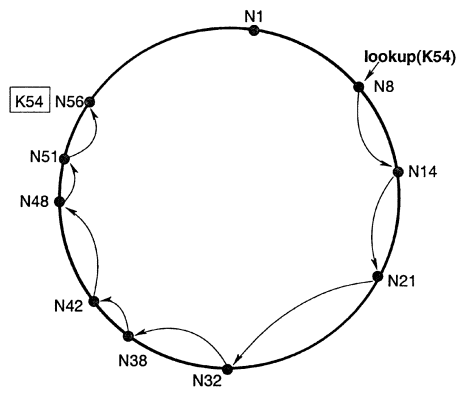
\includegraphics[width=5cm]{img/chord-lookup.png}
    \caption{Chord file query mechanism \cite{stoica2003}}    
    \label{fig:chord}
    \end{subfigure}
    ~
    \begin{subfigure}[t]{0.4\textwidth}
    \centering
    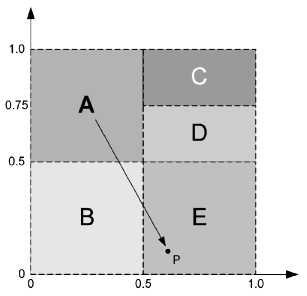
\includegraphics[width=5cm]{img/can-lookup.png}
    \caption{CAN file query mechanism \cite{p2p-survey-1}}
    \label{fig:can} 
    \end{subfigure}

\caption{Examples of structured P2P query mechanisms that utilize DHTs}
\label{fig:dht-usage}
\end{figure}

\subsection{Effects to the Network Infrastructure}

\label{ssec:p2p-effects}

    Historically, \glspl{isp} have deemed \gls{p2p} traffic as unideal or even undesirable.
    Besides the aforementioned illegality precedent that is tied to \gls{p2p} applications, the overall properties of \gls{p2p} networks make them unappealing to support - due to the distributed nature of these types of networks, the overall traffic is less predictable, with the higher upload traffic volume in edge networks requiring infrastructural investments, and the network-agnostic operation mode of \gls{p2p} applications leads to inefficient and uncooperative network resource usage.

    \gls{p2p} networks who neither have structure nor a central point of control have to utilize content retrieval methods which are bound to be less efficient than their counterparts.
    However, architectures which fit in these categories mostly do so with a clear purpose - Gnutella's decentralized nature makes it very hard for individual nodes or external entities to regulate what can happen in the network (such as enforce legal actions), and its lack of structure simplifies the implementation and reduces the overall effort to bootstrap to the overlay, making it a good fit for applications with a high peer churn rate.
    Similarly, FreeHaven, an also unstructured and decentralized \gls{p2p} protocol, has its architectural decisions fit a very specific use case, as it "emphasizes distributed, reliable, and anonymous storage over efficient retrieval" \cite{freehaven}.
    The lack of systematic means to efficiently locate content by these \gls{p2p} architectures means that more ad-hoc methods have to be used, which are less efficient and thus incur in bigger workloads for \glspl{isp} - the usage of query flooding by Gnutella and message broadcasting by FreeHaven are examples of this.

    The usage of structure by \gls{p2p} networks can, as stated before, result in more efficient content and peer location algorithms.
    However, maintaining such structure also requires a chunk of \gls{isp} resources, as peers need to periodically update other neighbouring peers, as well as react to them abruptly entering and leaving the overlay.
    The usage of key-value mappings with \glspl{dht} can also have the potential to be \gls{isp} unfriendly, as the hash function can be designed to evenly distribute resources over the peer pool, and thus over the network - whilst such property is certainly advantageous in certain use cases, doing so removes any application context that exists in the content - for example, grouping resources which belong to the same web page with such a method isn't efficient, as they will be individually hashed and spread throughout the network, despite the fact that they'll likely be requested together for each page access.

    A first point of improvement is optimizations made in the applications themselves to less degrade network resources.
    An example of these can be visualized in Figure \ref{fig:p2p-optimization}.
    Specifically, regarding Figure \ref{fig:chord2}, a point of optimization in the Chord system would try to reduce the number of query messages per resource by increasing the number of successors a given node knows.
    That way, the querying node can instead query not for the single successor it knows, but instead by querying for the one who's ID immediately precedes the content's, thus insuring a reduced number of hops to retrieve the message.
    This consequentially also reduces the total amount of traffic on the network, and improves application times.
    Regarding Gnutella in Figure \ref{fig:gnutella2}, a point of optimization would try to tackle the usage of query flooding to locate data, since such flooding grows exponentially and thus intakes a massive toll on network resources.
    A query flooding system would not be as prejudicial if content was equally scattered throughout the overlay and each given content was a minimal amount of hops away.
    However, as concluded by extensive analysis of user traffic on Gnutella during its heightened use, nearly 70\% of users shared no files and nearly 50\% of all responses were returned by the top 1\% of sharing hosts \cite{freeriding-gnutella}.

\begin{figure}[t!h]
    \centering
    \begin{subfigure}[t]{0.4\textwidth}
    \centering
    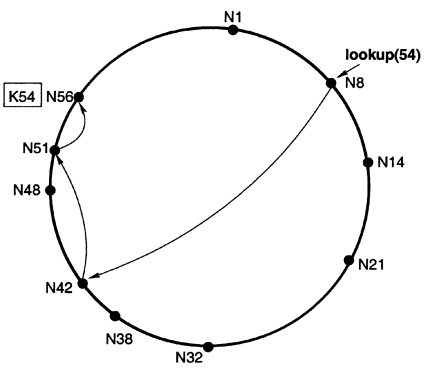
\includegraphics[width=6cm]{img/chord-lookup-efficient.png}
    \caption{Chord file query mechanism with more neighbours known per peer \cite{stoica2003}}
    \label{fig:chord2}
    \end{subfigure}
    ~
    \begin{subfigure}[t]{0.4\textwidth}
    \centering
    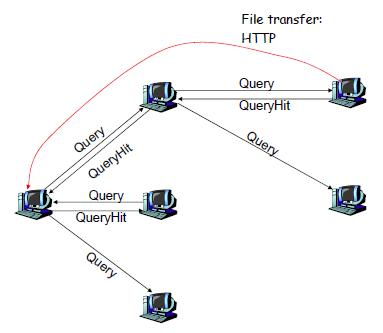
\includegraphics[witdh=6cm]{img/gnutella-flood-efficient.png}
    \caption{Gnutella file query mechanism assuming reduced resource-to-peer hop distance}
    \label{fig:gnutella2}
    \end{subfigure}
    
\caption{Examples of \gls{p2p} query mechanisms with application optimizations}
\label{fig:p2p-optimization}
\end{figure}

    Regardless of the many ways through which \gls{p2p} systems can operate, e.g., in regards to structural mechanisms and centralization, and even disregarding potential application optimizations, no classic \gls{p2p} system operates in full understanding of the underlying network topology, nor with a cooperative behavior towards \glspl{isp}.
    The network-agnostic manner under which they operate results in overlay networks which are layered on top of the underlay where they run, as exemplified in Figure \ref{fig:overlay-underlay} - as \gls{p2p} applications are network-agnostic, two neighboring peers could exist in completely different contexts on the common network layer - for example, they could either be connected by a single data link or be multiple network provider domains away from each other.

\begin{figure}[!h]
\centering
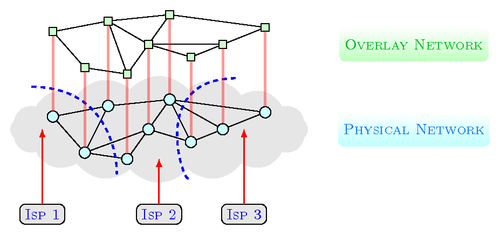
\includegraphics[scale=3.0]{img/p2p-topology.png}
\caption{Example demonstration of an overlay network and corresponding physical layer \cite{overlay-vs-underlay}}
\label{fig:overlay-underlay}
\end{figure}

    The inability of \gls{p2p} applications to localize traffic is seen as a big problem - as concluded by \cite{liao2014}, \glspl{isp} face bottleneck bandwidth pressure in the large scale Internet of the future, with it being in particular due to \gls{p2p} applications.
    However, an argument is made that an increase in users from such applications is not necessarily harmful, and perhaps helpful, if traffic locality can be boosted.
    Thus, there is value in ensuring that peers prefer to generate traffic within network locality over traffic that crosses network borders.

    A first step towards more traffic locality would be increasing the availability of content inside network boundaries, through means such as cache injections or peer content serving incentives.
    Given that content resides locally, a second step would be that \gls{p2p} applications have a network-aware vision of the overlay, which does not happen with classic \gls{p2p} protocols.
    This issue is particularly damaging in \gls{p2p} applications whenever neighbours are selected, and when deciding what peer or collection of peers to consume a given service from.

    If it is the case that \gls{p2p} applications are not locality aware, it can easily be seen how this can be an issue. In one hand, for the applications, choosing peers which are not local to the querying peer may result in more time to retrieve the requested contents. 
    In the other hand, for the \glspl{isp}, bad network resource utilization can incur in higher operational costs, and may degrade overall network performance in many cases, e.g., by not being able to stop applications from overusing inter-AS links, which usually are network bottlenecks (a conventional wisdom demonstrated in \cite{akella}) and which, due to peering agreements with other \glspl{isp}, are less desirable to be overused due to peering costs.
    If the \gls{p2p} application were to attempt to choose the peers that would most effectively serve the querying peer, it could depend on privileged information that the ISP has on the network's properties and current status, such as the inherent network topology, link properties, or scheduled server maintenances.

    Attempting to optimize peer selection without a co-operational channel with \glspl{isp} would be sub-optimal, as not enough information can be derived with network probing alone, and could perhaps even be more damaging with the wrong techniques - consider a peer selection algorithm that chooses the peers with lowest \gls{rtt} of a probing ping message, whilst having no indication on available end-to-end bandwidth, existing network bottlenecks, or peak traffic hours.
    Likewise, attributing neighbour pairings via geographical proximity, whilst initially seems like a good step in location awareness, may also not be optimal - \glspl{isp} may not always prefer geographical proximity in connections, as peers could be very geographically close but residing in different \glspl{as} and thus separated by costly links.
    Other peer-selection techniques focus on randomly selecting nodes, such as the means through which a BitTorrent tracker selects between redundant peers serving the same file chunk \cite{bittorrent-details}, which is simple and resilient to peer churn \cite{qin2009}, but as a consequence is sub-optimal on network resource usage as no network consideration exists.
    It is reasonable to assert that no \gls{p2p} application can act with full \gls{isp} consideration without directly cooperating with it, and simple heuristics should be, whenever possible, traded for methods where full cooperation with the underlay is done - that is, if the needs of both layers are being met.

    Indeed, it is the case that current \gls{p2p} solutions are \gls{isp}-unfriendly.
    More concretely, \cite{isp-p2p-tussle} shares the view that \gls{p2p} applications and \glspl{isp} are in a tussle, since \gls{p2p} applications generate traffic which favours the application's needs while ignoring those of the \gls{isp}, which in turn upsets the latter's business model.
    To name a few examples, BitTorrent seems to employ peer selection algorithms which do not consider the underlay network, which can result in degraded download performance and increased load on \glspl{isp} \cite{qin2009}.
    \cite{karagiannis} found that since this protocol is locality unaware, 70-90\% of content existing locally was found to be downloaded from external peers, and suggests that locality-aware content distribution algorithms could significantly reduce the total amount of traffic generated.
    Likewise, Gnutella generates traffic which is not ideal, as it may have to cross ISP network boundaries multiple times \cite{estimating-gnutella} due to the same fundamental issue stated before - an application layer that operates in disregard to the network underlay it runs on.

    As \cite{dan-Commag10} describes, the ongoing friction between the overlay and underlay layers has made it to the point where \glspl{isp} have chosen to throttle the bandwidth of \gls{p2p} traffic, or even outright block it.
    In return, \gls{p2p} applications have tried to mask their presence to bypass such restrictions via tunnelling or using non-standard and random port numbers.
    This is an unsustainable system that is bound to hurt both \gls{isp} profit and application functionality, and a strategy of cooperation between the overlay and underlay layers is crucial to guarantee that the requirements of both parties are met, specially in the face of the increased challenges contained in the Internet of the future.

\section{Content Distribution Networks (CDNs)}

\label{sec:state-cdn}

\subsection{Concepts and applications}

\label{ssec:cdn-concepts}

   A \gls{cdn}, as the name implies, is a network specifically designed with its main focus on distributing content to a set of end users.
   Its design allows for the alleviation of performance bottlenecks on the Internet generated by client requests, and has been recently considered a powerful tool as a response to the existing high demand for media content, which has a huge share of the global Internet traffic of today.

   Functionalities of \glspl{cdn} include \cite{cdn-survey}:

    \begin{itemize}
        \item \textbf{Content outsourcing and distribution:} Replicate content throughout the network into edge servers nearby end users.
            This allows \gls{cdn} clients to pay for their content to be hosted on these edge servers, and in doing so guaranteeing that it is quickly accessible by their own content clients.
        \item \textbf{Request redirection:} Direct a content request to the most appropriate edge server at a given time.
            This redirection is done considering relevant network properties, such as client and server geographical locations, as well as current server loads.
        \item \textbf{Content negotiation:} Manage the network's properties and allocate resources to fit the needs of its clients through negotiation.
        \item \textbf{Management:} Manage the distribution network, which includes accounting, monitoring, statistical analysis on content consumption, etc.
            A close management of the distribution network is important for its business model, as, besides being needed for a billing system, allows for a better understanding of the networks' usage patterns, which is helpful information for better engineering the system to most optimally serve content with increased revenue and decreased costs.
    \end{itemize}

    The current focus of \glspl{cdn} is thus to provide content, e.g., web pages, documents, photos, videos, or media-related streams, with high availability and performance.
    The strategy used by them to guarantee a satisfying \gls{qoe} on a global scale is the deployment of content close to the end-user - a \gls{cdn} contains many nodes which are geographically spread throughout the globe and close to the users they wish to serve, and whenever such users request for content, they are routed to the node which is closest to them \cite{cookbook}.

    Data replication to servers which are strategically placed closest to end-users, coupled with good means to properly redirect such users to the most attractive edge server, is what allows content to be available more often and more quickly.
    These are undoubtedly attractive features in the world of e-commerce, where user \gls{qoe} can dictate much of the profit - for example, Akamai, one of the leaders in \gls{cdn}-related services, ran a research concluding, among other things \cite{akamai-retail-report}:

\begin{itemize}
    \item A 100 millisecond slower web page loading speed can result in a 7\% drop in sales
    \item A 2 seconds slower web page loading speed can almost double the number of visitors who end up abandoning their carts
    \item 53\% of users who use smartphones to visit web stores won't make the sale if the web page takes more than 3 seconds to fully load
    \item 28\% of users won't return to the same web store if they think it takes too long to load
\end{itemize}{}

    It should then come as no surprise that streaming services such as Netflix or Youtube, who now reach a global scale and whose utility is highly dependant on their high availability and low transmission delay, routinely use \gls{cdn} solutions.
    More broadly, typical \gls{cdn} customers include media and Internet advertisement companies, data centers, \glspl{isp}, online music retailers, mobile operators, etc \cite{cdn-survey}.
    Indeed, companies that wish to provide a given service in the web at scale routinely partner with companies whose focus is providing content delivery services, with popular examples being Akamai, CloudFlare \cite{cloudflare}, or Amazon Cloudfront \cite{cloudfront}.
    Coupled with the promise of highly available and quick content retrieval, these companies also provide other attractive services, such as firewalls and \gls{dos} protection.

    The Internet's currently most targeted use being media consumption has made it so \glspl{cdn} and their providers have an important role in dictating a very considerable percentage of traffic flow in \gls{isp}-owned infrastructures, and as such their study and improvement is quite important.
    With their great influence over global traffic, active efforts should exist to increase harmonious behaviours between applications that utilize their services and the \glspl{isp} that support it, with the goal in mind being network resource efficiency to guarantee that the infrastructure can remain operational and applications can provide a satisfiable user experience.

\subsection{Architecture}

\label{ssec:cdn-architecture}

    Figure \ref{fig:cdn-conceptual-architecture} represents a high-level conceptual architecture of a \gls{cdn}.
    The true power of these kinds of networks comes from their strategically deployed cluster of replicated servers - at a global scale, this implies having them geographically dispersed and located inside or nearby networks with large content demands.
    The origin server possesses the content that is to be served, and the bootstrapping process has the content uploaded into the network, which is afterwards replicated to these edge servers.

\begin{figure}[!h]
\centering
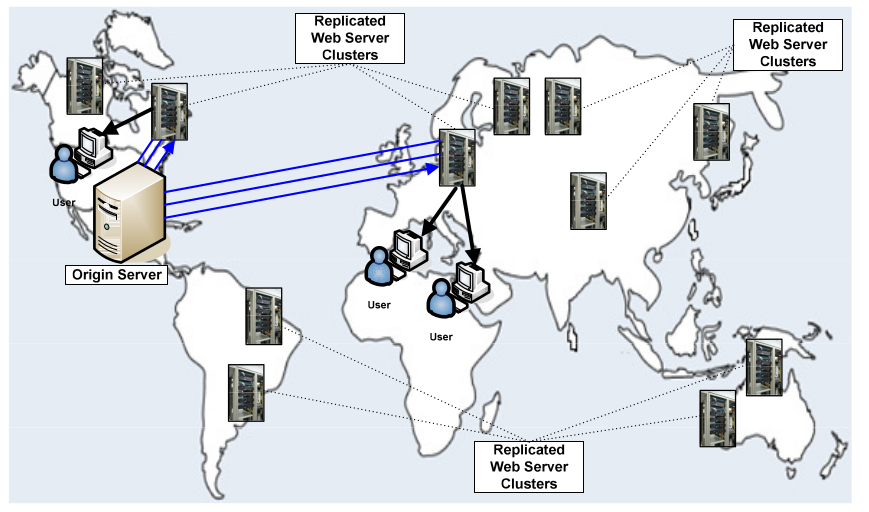
\includegraphics[scale=0.50]{img/cdn-architecture.png}
\caption{Conceptual architecture of a \gls{cdn} \cite{cdn-survey}}
\label{fig:cdn-conceptual-architecture}
\end{figure}

    Figure \ref{fig:cdn-request-routing} displays how, conceptually, the request routing functionality of a \gls{cdn} works.
    As can be seen, the request is firstly directed to the origin server, which serves only light and basic content.
    In the situation where large static content is requested, the origin server redirects the request to the \gls{cdn} provider, which utilizes a selection algorithm to elect the most appropriate edge server to serve the content to the end user.

\begin{figure}[!h]
\centering
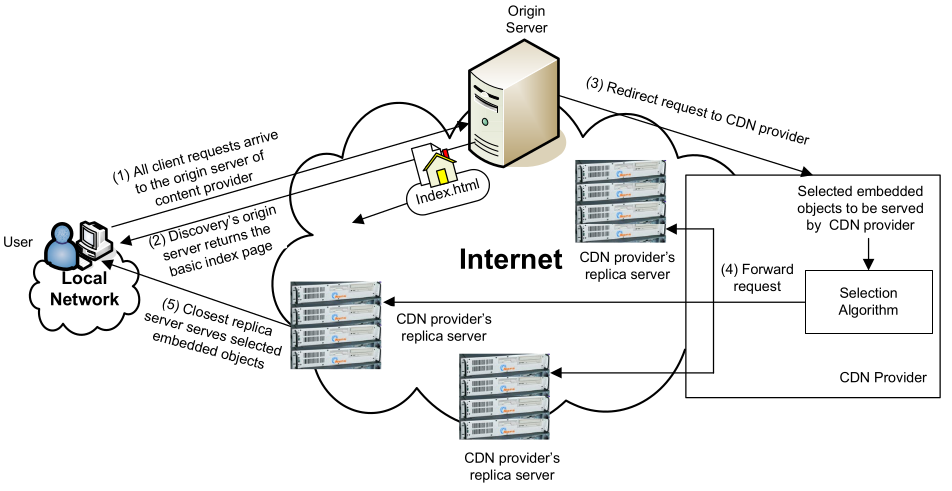
\includegraphics[scale=0.50]{img/cdn-request-routing.png}
\caption{Request routing functionality of a \gls{cdn} \cite{cdn-survey}}
\label{fig:cdn-request-routing}
\end{figure}

    The request routing mechanism is the one that redirects a given user to a given edge server.
    The prevalent approaches are, according to \cite{wichtlhuber2017}, the following:

\begin{itemize}
    \item \textbf{\gls{dns} request routing}: The user must first resolve a domain name to retrieve a piece of content. The \gls{cdn}'s \gls{dns} server processes the request and, utilizing the user's \gls{ip} address, historical measurement information and current server loads, responds with the address of the edge server that seems most fitting to provide such content.
    \item \textbf{\gls{http} request routing}: Content is firstly requested to a nearby proxy server, which in turn answers with an \gls{http} redirect to be resolved by the client in order to find the content.
        The \gls{http} requests can occur in subsequent rounds and can also use \gls{dns} knowledge when the redirection domain must be resolved.
    \item \textbf{Anycast request routing}: The \gls{cdn} provider announces an anycast prefix to the network.
        Whenever a router receives multiple announcements to the same prefix incoming from different locations, it chooses one considering some custom criteria, usually being \gls{as} hop count and \gls{igp} weight.
        Thus, different routers can have a given anycast address mapped to different hosts, meaning the ones that are most suitable for that particular router.
\end{itemize}

    These mechanisms are also discussed in \cite{cdn-survey}, but also add:

\begin{itemize}
    \item \textbf{\gls{gslb}:} Service nodes, consisting of edge servers and \gls{gslb}-enabled web switches, are interconnected in a network.
        Individual nodes possess global awareness of the network, meaning the status of each individual server.
        With edge servers having more information on the health and status of all other candidate edge servers, and the web switches acting as authoritative \gls{dns} servers, the network can enable the support of a global-wide server load balancing mechanism that intakes dynamic server information.
    \item \textbf{\gls{url} rewriting:} The origin server redirects the end user via dynamically altering the host pages' \gls{url} links.
    \item \textbf{\gls{cdn} peering:} An extension of a single \gls{cdn} network to multiple, interconnected \glspl{cdn} which serve content on behalf of others when appropriate.
        This is helpful to extend the domain reachability of a single \gls{cdn}, increase fault tolerance, and ability to achieve better performance with more candidate servers to choose and balance loads from.
\end{itemize}

    It is vital that a \gls{cdn} possesses a clear view of the network performance inside its domain.
    \cite{cdn-survey} lists important metrics which are used to measure \gls{cdn} performance:

    \begin{itemize}
        \item Geographical proximity of end users
        \item Path latency
        \item Path packet loss
        \item Path Bandwidth
        \item Path startup time
        \item Path frame rate
        \item Server load
    \end{itemize}

    Means through which these metrics are retrieved by the network include traffic monitoring of end user to surrogate server communications, and surrogate server feedback retrieval via application requests or measurement probings \cite{cdn-survey} \cite{akamai-report}.

    Having a clear understanding of CDN performance is important for system management in two fronts - firstly, through performance evaluation, by providing the billing and monitoring modules the verification of how the network is faring at its task of caching and delivering content on behalf of clients; secondly, through performance optimization, by providing the logical layer an updated view on network status, serving as contextual input that the system uses to better reason on how to act - for example, in regards to the caching and request routing mechanisms.

\subsection{Effects to the Network Infrastructure}

\label{ssec:cdn-effects}

    As previously discussed, \glspl{cdn} came as a tool to strategically position content on the network in such a way that it can more quickly and more reliably be retrieved by an end-user.
    These \gls{cdn} systems are then inherently a mean of optimizing network resource utilization in the application layer, and thus are of great interest for \glspl{isp} and, if done properly, can be very appealing not only to them but also to end-users that use applications leveraging these networks.

    The usage of a single content-providing server - or a limited set of them - which is far away from the content demand, that in turn has a large geographical distribution, is prone to server overloading and path congestion problems if a big enough scale is achieved.
    Data caches are a classic solution to network inefficiency problems, and are used by \glspl{cdn} as a means to replicate content to strategic locations to better serve users, with the added benefit for \glspl{isp} that their network resources are efficiently used, with the ability of reducing the total amount of used bandwidth needed for a service to operate - as data travels a shortened total amount of network hops from data source to points of data demand - and reducing congestion of inter-domain links - as data caches will reside locally and redistribute traffic away from highly shared network links.
    It can thus be stated that the relationship between \glspl{cdn} and \glspl{isp} allows for a win-win scenario because efficient network usage has consequentially better service quality, benefiting service providers and applications, respectively.

    However, \glspl{cdn} seem to lack cohesion with the underlying network infrastructure during normal application operations.
    As stated by Akamai, a leader in \gls{cdn} services, in their report \cite{akamai-report}, the large scale and complexity of the Internet, where it takes well over 650 networks to reach 90\% of all access traffic, adds to it many challenges to the \gls{cdn}'s role of content delivery.
    In particular, whilst good investment seems to exist at the first and last mile of Internet access (server and end user placements, respectively), there seems to be little economic incentive to invest in the middle mile, composed of peering points shared among networks.
    These peering points then become network bottlenecks that are susceptible to increased traffic packet loss and latency, making inter-network communications unreliable, and loose coordination between autonomous networks with internal biases is pointed as a main cause.
    Due to this, even a well provisioned data center will be at the mercy of the various inter-network bottlenecks that may arrive, and performance is susceptible to degradation.
    In fact, the paper suggests a clean-slate redesign of the Internet as a potential solution to its many problems - besides the peering point congestion mentioned above, inefficient routing protocols, unreliable networks, inefficient communications protocols, and application limitations also add to the problematic - but such a redesign to a massive and highly critical global infrastructure doesn't seem feasible.

    In alternative to proper network infrastructural insight, \glspl{cdn} have to rely on network probing, traffic monitoring, and server feedback, as discussed on Section \ref{ssec:cdn-architecture}.
    Even assuming that these are sufficient, the usage of probing techniques will incur in overhead traffic on the network, with this overhead being exacerbated if many other overlay networks or applications also apply this technique.
    Similarly, traffic monitoring to extract end-to-end path metrics to end users requires resources and takes time, and may also incur in redundant operations being applied on the network.

    Advantageous as network probing and traffic monitoring mechanisms can be for \glspl{cdn} to properly conduct request routing and caching decisions, a case must be made for proper application-infrastructure synergy during decision making in the overlay.
    Much like \gls{p2p} systems, to infer on network status by measuring it is insufficient when compared to receiving input from trustworthy and authoritative entities that possess privileged network information, such as \gls{isp} administrators.
    Attributing node pairings entirely on geographical data was previously discussed as being a non-optimal way of assessing node selection at the application layer in Section \ref{ssec:p2p-effects}, and the same would apply in the case of \glspl{cdn}, where edge servers are paired with end-users.
    Again, much like in the scenario of peer selection in \gls{p2p} systems, the usage of network measurements made by the \gls{cdn} itself to better pick the appropriate end-server, while potentially beneficial, can certainly be improved upon if it used additional, hard to retrieve data that only \glspl{isp} or other privileged infrastructural entities could possess, and which are at position to guide applications in the infrastructure they deeply possess knowledge on.

    There indeed seems to be a consequential coupling between overlay decisions in the \gls{cdn} systems and the underlying infrastructure.
    If the \glspl{cdn} were not to take \gls{isp} input when redirecting clients, suboptimal choices would be made that would be prone to bottleneck congestion, and if, in the other hand, \glspl{isp} were to employ only their own biases in content request redirection, user-level application \gls{qos} agreements might not be met.
        \cite{pushing-cdn-isp-collaboration} states that this lack of awareness to network status is indeed problematic for \gls{cdn} systems, listing end-user mismatching to edge servers based on dubious \gls{dns}-based location binning and resource consuming, non exact methods to detect bottlenecks, as well as lack of agility in server deployment in ideal locations.
        This is a view shared by \cite{cdn-isp-cooperations}, which adds that these problems reside in a shared medium that raises the opportunity for cooperative behavior that would enable better application performance and optimized \gls{isp} resource utilization.
    In fact, Akamai themselves have formed content delivery strategic alliances with major \glspl{isp}, with AT\&T \cite{att}, Orange \cite{orange}, Swisscom \cite{swisscom} and KT \cite {kt} among them \cite{pushing-cdn-isp-collaboration}, which hints at this type of partnership being the norm for content distribution technologies of the future.

        \gls{isp} input permits applications to act in a more network-aware fashion than without it - whereas pairing overlay nodes or deploying edge servers in terms of geographic distance, \gls{rtt} distance, or any other metric, may give further decision power than a purely network-agnostic overlay system, proper guidance by \glspl{isp} could help pairing based on more complex metrics that, besides the aforementioned ones, also consider ISP objectives, e.g., to minimize network distance, avoid bottlenecks, locate content caches, etc.
        A more efficient Internet can be obtained if many other overlays coordinate their efforts with the \gls{isp}, which in turn can now orchestrate its traffic in a way that would previously be generated with no prior guidance, and that can now be engineered to maximize network resource utilization and, consequently, application performance.

\section{Client-Server Model}

\label{sec:state-client-server}

\subsection{Concepts and applications}

    The Client-Server model is a classical way of attributing roles in the network.
    Whereas the \gls{p2p} architecture blends server and client roles into each node, this architecture delineates two distinct ones - the client and server - and their purpose on the network, as Figure \ref{fig:cli-serv-architecture} shows.
    With it, the service layer is centralized onto the server nodes, and the only role expected of client nodes is to request services from them.
    Operating with philosophies which are opposite to the \gls{p2p} architecture, it is to be expected that the advantages and disadvantages should too be contrasting - by centralizing the services, maintenance and general administration of serving nodes are much facilitated, and limiting the number of servers to a select and trustworthy few, instead of scattering that functionality to all nodes in the network, greatly minimizes security risks.
    On the other hand, the drawbacks are also apparent and mirror a distributed solution - issues of scalability, resilience to failure, and resilience to monopolization of power arise from the decision to engineer an application that creates clear boundaries between client and server.

    \begin{figure}[!h]
    \centering
    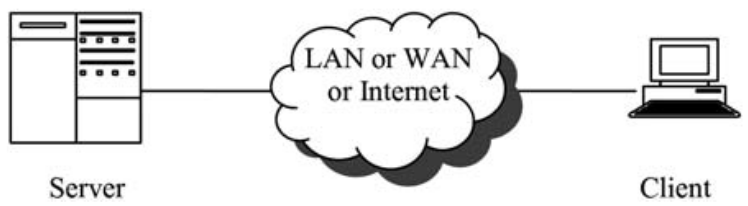
\includegraphics[scale=0.55]{cli-serv-architecture.png}
    \caption{Client-Server architecture \cite{cliserv-p2p}}
    \label{fig:cli-serv-architecture}
    \end{figure}

    This classic architecture has seen a lot of adoption by applications, with use cases that include serving content via \gls{http} or \gls{ftp}, or enabling e-mail communications \cite{cliserv-p2p}, to name a few.
    Adding to this, the client-server approach also serves as a direct alternative to the \gls{p2p} one in many fields, e.g., file transfer or media streaming, with their respective advantages and disadvantages needing to be weighted out for a proper choice to be made.

    As an attempt by service providers to still operate a client-server model whilst reducing its associated downsides, given techniques were created and employed.
    One of which, by the name of \gls{cdn}, is of particular importance in this work and as such has its specific overview in Section \ref{sec:state-cdn}.
    Some other methods will be discussed below.

    Server mirroring, one famous technique, is the act of continuously synchronizing a server into its replica, or mirror, essentially creating an exact copy of it that is now accessible as if it were the original.
    Whilst \glspl{cdn} aim at replicating chunks of contents wherever it may be necessary, the act of server mirroring performs an integral copy of a server which is self sufficient at servicing a given client, as long as it periodically checks up with the primary server for synchronization.
   It is a standard business strategy that uses redundancy as a means to increase reliability, availability and performance.
   The existence of many servers that perform the same task means that these can be strategically chosen to serve a client in a given situation, e.g., by selecting the one that has reduced load and smaller end-to-end message delay to the user.
   Figure \ref{fig:mint-mirrors} shows an application of this, where multiple server mirrors exist to deliver software packages to the Linux Mint \cite{linux-mint} distribution.
   The user has the choice to manually select one of these mirrors, and ideally chooses the one that is most fitting to them.

    \begin{figure}[H]
    \centering
    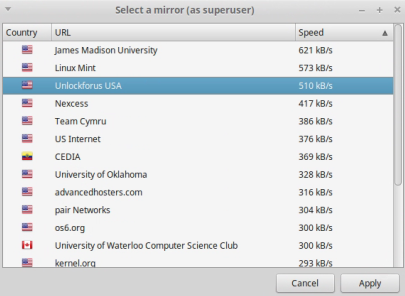
\includegraphics[scale=0.8]{mint-mirror.png}
    \caption{Linux Mint prompt to select a software repository mirror}
    \label{fig:mint-mirrors}
    \end{figure}

    Server load balancing is another popular technique to solve scalability issues, and it refers to the act of distributing tasks over a set of computing nodes as a means to make the service more efficient, since a server with little processing load is bound to respond quicker than one with more, and situations of overloading become less common as it is now spread out over multiple processing units.
    Load balancing algorithms can be categorized, according to \cite{load-balancing}, in two categories:

    \begin{itemize}
        \item \textbf{Static}: Does not take current system status into account, instead acting upon static rules that define the load type, in regards to, for example, processing power and memory requirements.
            A round-robin or random selection of load attribution are part of a static approach.
        \item \textbf{Dynamic}: Load is distributed at run time, considering dynamic information about the system that is continuously being collected.
    \end{itemize}

    A static approach can be compelling due to its simple nature that makes it easy to implement and much faster in comparison to run.
    On the other hand, a dynamic approach is more complex by definition as it requires the additional infrastructure required to collect and compute upon the system statistics.
    As it might be expected though, a load balancing scheme that attempts to optimize resource utilization considering real-time information about system status and performance is bound to have bigger potential at effectively selecting which server should handle a given request, since more factors are known to better aid the decision, including the current server loads in the server cluster, their available resources, network conditions, etc.

    Several methods exist through which to implement load balancing.
    For example, \gls{dns}-based approaches perform the load balancing at the domain name resolving stage, where the IP address response is given after selecting an optimal server, such as the proposal in \cite{dns-load-balancing}.
    \gls{sdn} solutions, as another example, leverage a control pane that is responsible for intercepting server access calls and activate the load balancing mechanisms that redirect that call to the selected server, as happens in the proposal in \cite{sdn-load-balancing}.


\subsection{Effects to network infrastructure}

\label{ssec:client-server-effects}

    As a base method, the utilization of the client-server architecture is not at all recent to \glspl{isp}.
    Quite the contrary, it was the norm throughout the decades to provide a service by using a set of single-purpose server machines.
    Intuitively, using a limited number of servers to respond to client needs will have problems scaling, as increased demand is prone to service overload and path congestion, hence the need to employ some of the strategies discussed on the previous section.
    These strategies come from the necessity to fulfill both application and \gls{isp} requirements, i.e., to achieve proper \gls{qos} levels and infrastructure resourcefulness that helps the general good function of the network, respectively.

    Much like the content replication utilized in \glspl{cdn}, an integral replication of a main server proves itself as an advantageous tool capable of delivering services more closely to users, and as such allows the reduction of total amount of bandwidth used to serve all clients.
    Optimizing application traffic is crucial to guarantee good network resource usage, and in case of server mirroring it comes down to good strategic deployment and dynamic, intelligent algorithms to properly attribute mirrors to requesting end-users.

    Giving end-users the choice to manually select the serving mirror, as commonly happens when downloading software, for example, seems problematic, as application-generated traffic is not optimized.
    In fact, when considering the Linux Mint software package distribution discussed in the previous section, despite there currently existing seventy mirrors deployed throughout the globe to fit this role, a large number of these remains mostly unused whilst the main and default server is constantly prone to overworking \cite{mint-article}.

    It can be stated that end-users both don't care enough to optimize traffic nor do they have enough information to properly do so even if they did.
    Deployment of server mirrors is a great tool that brings with it the issue of optimizing server selection, and much like all examples given so far, traffic generated by applications can be firstly optimized by the applications themselves if they consider static and dynamic information of the network they operate on.

    Load balancing is too a point of great interest in the task of application-layer traffic optimization.
    The task of attributing a current request to a pool of available redundancy workers is a common strategy to help scalability, and the means through which to do so have concrete network consequences, since it has the power to shape great amounts of traffic in ways that can be more or less preferable for \glspl{isp}.
    It could then be deduced that a load balancing strategy has better chances of being efficient if it fully aware of both server status and network conditions.
    Doing so with \gls{isp} cooperation would reveal insight into some network status information and administrative preferences.
    For the section of data that could be retrieved utilizing probing and measurement strategies, a bank of centralized data possessed by an entity with full network knowledge would greatly reduce overhead probing traffic and monitoring computation cycles.
    For the section of data that could only be retrieved with proper \gls{isp} insight, more efficient and network-cognizant decisions would now be possible, in contrast to the limited one-sided attempt at optimizing application decisions that generate traffic.

\section{Traffic optimization by applications and layer-cooperative approaches}

\label{sec:state-solutions}

    This section serves to display proposed solutions and existing implementations that have been made in the attempt to optimize application traffic utilizing network information.
    Given the increasing scale of the Internet as a near ubiquitous system, and the increasing tension between applications and service providers, it comes as no surprise that the area of layer cooperation has been through exhaustive work.
    Many solutions have been devised for specific use cases, with varying degrees of power given to each one of the layers, and different levels of cooperation.
    Along with their description, their review is made in regards to what the proposals state their impact is to applications and the infrastructure, as well as the accompanied advantages and disadvantages.

\subsection{Peer-to-peer applications}

\label{ssec:approaches-p2p}

    Many different mechanisms have been developed with the goal of decreasing tensions between \glspl{isp} and \gls{p2p} applications, which is a subset of the general layer cooperation problem.
    Figure \ref{fig:p2p-isp-interactions} represents a grouping proposed by \cite{dan-Commag10} where such mechanisms are ordered in agreement with how much involvement the \gls{p2p} systems and the \glspl{isp} have. 

    \begin{figure}[H]
    \centering
    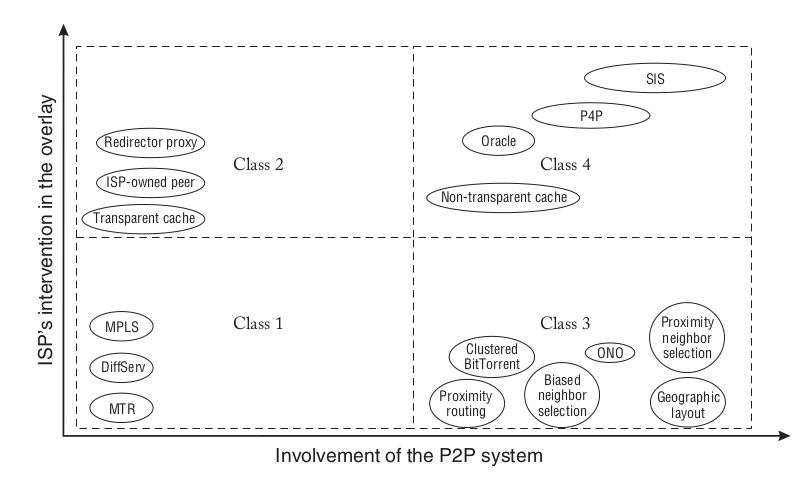
\includegraphics[scale=0.65]{img/approaches-isp-p2p.png}
    \caption{Approaches to decrease tension between \gls{p2p} applications and \glspl{isp} grouped by their involvement \cite{dan-Commag10}}
    \label{fig:p2p-isp-interactions}
    \end{figure}

    In a more detailed fashion, these classes are as follows:

    \begin{itemize}
        \item \textbf{Class 1}:
            There is not much - or any - interference in the overlay by \glspl{isp} nor are \gls{p2p} systems cooperative.
            Instead, \glspl{isp} apply traffic engineering methods to selectively favour types of traffic.
            This is usually done to guarantee certain \gls{qos} levels to some classes of traffic, which are then to be treated favourably at the forwarding and routing levels.
            Examples of such techniques are \gls{diffserv}, \gls{mtr} and \gls{mpls}.
            These classes of methods do not fix the underlying application behaviour, but are instead used to control preexisting traffic.
            As such, the peers' routing decisions are not affected and \gls{p2p} traffic still remains non localized.
        \item \textbf{Class 2}:
            There is \gls{isp} intervention in the overlay in such a way that peers continue normal operations without realizing that such interventions occurred.
            This can be reached via the use of proxies that can affect the control plane with the redirection of content requests to local peers, or at the data plane with content caches which act as normal peers and are strategically placed in the network.
            These methods are advantageous because they do not require any changes to the \gls{p2p} protocols, since the \gls{isp} has an active role in molding to the overlay, intercept traffic, and either help or guide it in a way that favours them.

            Class 2 techniques haven been proven to work , as concluded in \cite{dan-Commag10}, and put into practice, for example, in \cite{programmable-trackers}, \cite{configurable-trackers}, and \cite{rev3}, via the specification of a BitTorrent tracker that is programmable to allow for \gls{p2p} qualitative differentiation and \gls{isp}-cooperative traffic engineering that could help reduce inter-domain traffic significantly.
            Additionally, in \cite{altruistic-gnutella}, with the injection of special nodes on the Gnutella overlay which interface with the base protocol nodes but with the added caching and load-balancing mechanisms, in the attempts to alleviate the great amount of "free riding" that exists in Gnutella applications - as discussed in Section \ref{ssec:p2p-effects} - by minimizing the total amount of query floods and more evenly distributing content throughout the network for increased infrastructure resourcefulness.

            Despite their proven results in many areas, this class of mechanisms is not without its challenges - firstly, it involves much effort by \glspl{isp}, as it requires structural upgrades and constant adaptiveness to new and changing \gls{p2p} protocols.
            Perhaps worse, even when considering proper budget and maintenance, such methods can prove themselves to not be possible at all - for legal reasons, as data caches could possibly contain illegal content; and for technical reasons, since the packet inspection required by \glspl{isp} to detect and steer \gls{p2p} traffic may be blocked due to the peer's attempts to mask its traffic.
            It's also important to note that since no application-layer input exists, this approach could be one-sided in the sense that only \gls{isp} needs are favored without directly considering application needs.

        \item \textbf{Class 3}:
            Relative to a class 2 approach, the active role is switched and it is the \gls{p2p} system itself that acts in regards to the underlay it operates on, but without \gls{isp} involvement.
            Peers probe the neighboring network elements as a way to get more familiar with connection properties, and act on these probings during operation, e.g., when choosing neighbours to construct the overlay network with, or when choosing from whom to request a given resource.

            Whilst these methods can be advantageous for both applications and \glspl{isp}, it can't be assumed that to always be the case - as peers have no \gls{isp} input, they cannot have a full knowledge scope of the network and its needs, and as such these application optimizations can end up being more hurtful than helpful.
            For example, consider a scenario where a peer uses \gls{rtt} measurements to choose between two candidate peers, but the one that is the least round-trip time away from him belongs to another \gls{as}, and his preference for it to supply the service would incur in more infrastructural costs.

            The paper describes this class as a "win-not-lose" situation, meaning that while the \gls{p2p} system can, in the right circumstances, improve their performance via measurement-oriented strategies, the ability to act in a way that positively affects the underlay, without any feedback from \glspl{isp}, cannot be guaranteed.

            Such an example of class 3 mechanisms could be seen in \cite{qin2009}, which improved BitTorrent's download performance and even managed to reduce \glspl{isp}' backbone and cross-\gls{isp} traffic.
            The technique consisted of having peers send traceroute measurements to the tracker, which in turn grouped the peers into local, intra-\gls{isp} and inter-\gls{isp} groups, with the assumption that inter-\gls{isp} links generally have much more latency than the rest.
            As peers would later query the tracker for content, the returned peer list would be biased in such a way that promotes traffic locality.
            Another example of this is found in \cite{kim2011}, which devised a \gls{cdn}-\gls{p2p} hybrid where peers utilize \gls{rtt} measurements to group themselves by separate orders of geographical proximity with the same intent of the previous example, which is to localize traffic whenever possible.
            This technique also proved itself to be advantageous, as the solution was more efficient in terms of reduced total service disruption time when compared to a previous iteration of the hybrid architecture which used random peer selection to look up available target peers.
            As a final example, \cite{topology-aware-p2p-server-selection} proposed a node binning scheme that groups nodes of similar orders of magnitude of \gls{rtt} values to pre-defined landmarks, and utilized such scheme for topology-aware overlay construction mechanisms in some unstructured and structured \gls{p2p} overlays.
            Results allowed to conclude that even surface-levels topological information is advantageous and can significantly improve application performance.

        \item \textbf{Class 4}:
            Full and active cooperation exists between the \glspl{isp} and \gls{p2p} systems.
            The role of the \glspl{isp} is to provide information and guidance, and \gls{p2p} systems let themselves be influenced during operation.
            It is the methodology that most comes close to a mutually advantageous scenario for both parties, given that they both keep the entire group's needs in mind.

            For example, \cite{locality-aware-p2p} proposes an oracle that receives as input a list of candidate peers that the querying peer is considering connecting to, and ranks them by client connection proximity.
            Such method was tested in a simulated environment and proven to decrease negotiation traffic and improve scalability of \gls{p2p} networks.
            The functional intent of the oracle pattern is that he possesses privileged network information and acts on it to provide guidance to querying applications, and thus has the power to impose policies and optimizations unto applications, e.g., pair peers which are the least number of network hops apart via a Dijkstra algorithm using link costs derived from network-related ISP insight.
            Another approach that is the oracle proposed in \cite{han2009}, containing algorithms to dictate peer selection, task assignment and rate allocation.
            The method requires the full network topology as input - including link capacities and peer service costs - to minimize file downloading time and cost.
            The oracle would also be free to enforce \gls{isp} biases as preferential by modifying such algorithms to, for example, minimize usage of costly links (such as inter-\gls{as} ones, and subject to peering agreements).

            The \gls{alto} working group - whose work this thesis attempts to materialize into a working system and further extend its features - was formed to standardize the oracle-user scenario so it could be properly used in many situations at the scale of the Internet.

    \end{itemize}

\subsection{Content Distribution Networks}

\label{ssec:cdns}

    Given the current share that \glspl{cdn} have on the global Internet traffic of today, coupled with the demand for a good \gls{qoe} by end-users, this application domain has also been through efforts to optimize its traffic.
    One such way to do so is to optimize client query redirection, i.e., better choose which edge server should be attributed to an end-user when a name resolution is requested for some content.

    \cite{gromov2014} considers a \gls{cdn} built to deliver video data where some given set of content exists redundantly in many edge-servers, and presents an algorithm where the choice is made to optimize client download time, which in turn has to consider the network parameters at time of request, as well as current server load.

    Some simple, flexible and scalable techniques exist that utilize no ISP input.
    For example, \cite{topology-aware-p2p-server-selection}, mentioned in Section \ref{ssec:approaches-p2p} for its \gls{p2p} overlay construction with a binning technique based on \gls{rtt} measurements to landmarks, also utilized such binning technique for improved server selection.
    Similarly, \gls{ietf} tackled application traffic optimization via multi-\gls{cdn} cooperation, and devised a problem statement in regards to \gls{cdni} \cite{cdni-problem-statement}, which outlines the efforts required to specify a set of interfaces that allow for the interconnections of many \glspl{cdn}, with the added benefits that a multi-\gls{cdn} system, over an individualistic one, will have better properties, e.g., in regards to availability, coverage, and supported capabilities, as well as better \gls{qoe} for the end user, and reduced delivery costs for the service providers.
    The four devised interfaces - \gls{cdni} Control interface, \gls{cdni} Request Routing interface, \gls{cdni} Metadata interface, and \gls{cdni} Logging interface - are all to be operated at the application layer, and the group states that no new application protocol needs to be devised.
    Instead, existing protocols could be leveraged, e.g., \gls{http}, Atom publishing protocol, \gls{xmpp}, and in particular to the \gls{cdni} Request Routing interface, the \gls{alto} protocol could enable \gls{cdn} server footprint retrieval.

    Centralized network measurement repositories for wide consumption were tackled in projects such as \gls{idmaps} \cite{idmaps} and \gls{gnp} \cite{gnp}, that describe architectures for a global distance estimation service, leveraging measurements made by specialized nodes that retrieve raw network data, and heuristics provide scalable and functionally reliable path costs in metric such as bandwidth and latency.
    These consist of systems that centralize and share network probing results to querying entities, thus minimizing overhead traffic on the network.
    Such advantage goes outside of the \gls{cdn} realm, being useful for any overlay-residing application that wants to utilize network probing to be more underlay-aware for application optimizations.

    \cite{cdn-isp-cooperations} argues for the advantage of \gls{cdn}-\gls{isp} cooperative interactions and overviews three possible strategies that will be now discussed briefly: \gls{padis} \cite{pfa-10} is a system deployed and controlled by \glspl{isp} that monitors the network by listening to \gls{egp} and \gls{igp} messages and contains a privileged view of the topology and its status.
    It provides a service that ranks host-client pairs in regards to, for example, delay, bandwidth, or hop count, and experimental testings concluded that the download times of content provided by \glspl{cdn} that utilize \gls{padis} could be improved up to a factor of four, and generally gives much flexibility for \glspl{isp} to engineer traffic; \gls{cate}  \cite{fps-12} is designed in a similar manner to \gls{padis} but requires no client-side configuration, and experimental results concluded that network wide traffic was reduced by 15\%, link utilization was reduced by 40\%, and user-server performance generally increased; \gls{netpaas} \cite{pushing-cdn-isp-collaboration} was devised to fulfill two key enablers in a fruitful \gls{cdn}-\gls{isp} collaboration - user-server assignment, as it was tackled in the previous two examples, and server allocation, i.e., where should a \gls{cdn} deploy its servers their contents.
    This service, besides having the advantages of increased application performance and better \gls{isp} traffic control that were also mentioned in the previous two solutions, also facilitates the task of server allocation for \glspl{cdn}, reinforcing the discussed advantages and further optimizing \gls{cdn} operations.

    Still in the topic of \gls{cdn}'s edge server selection, \cite{wichtlhuber2017} suggests an \gls{sdn}-oriented solution that combines the performance of \gls{dns} load balancing with the low management overhead of \gls{ip} anycast.
    Load balancing is performed at the \gls{sdn} control layer by applying collaborative efforts between the \gls{cdn} and the \gls{isp}.
    This example of layer cooperation can allow for many optimization opportunities that leverage an existing and low-maintenance mean of request routing with the flexibility of \gls{sdn} solutions.

\subsection{Server-client applications}

    Attempting to optimize web server selection, \cite{kenichi} argues that \gls{dns}-oriented solutions, which select the nearest server but also employing load balancing, may not be the best at optimizing server-client \gls{qos} levels.
    Instead, it proposes a selection based on \gls{qos} measurements, from which three types are distinguished: a static method, such as choices based on least number of hops to server (which is unlikely to change); a dynamic method, consisting of network probing to assert, for example, \gls{rtt} values to the servers; and statistical methods, which decide based on a larger set of measurements previously made in various points in time.
    Utilizing the latter method, \gls{rtt} measurements and web-related request benchmarking is made, such as time to establish a \gls{tcp} connection, elapsed time from an \gls{http} GET method to first packet received, time to retrieve data fully, etc, every five minutes and spanning several weeks.
    The work concluded that statistical methods used to select between multiple equal web servers had high correlation with download time from the selected server, but optimizations should be evaluated in regards to computer workload and the amount of probing traffic.

    Tackling a similar challenge, \cite{swain} proposes a method of server mirror selection which is better optimized than the more popular approach of giving the user the selecting choice.
    The proposed solution's architecture consists of two types of agents: a client agent, which monitors the mirror server it was deployed in and stores static information, e.g., geographical location of server and maximum capacity, and dynamic information, e.g., current load and bandwidth.
    This information is then sent to the other role of the architecture, the server agent, which compiles it and acts as an oracle that is queried by users whenever mirror selection is needed, replying with a ranking of candidate servers based on bayesian networks.

    Congruent to the task of optimizing network traffic with layer cooperation, \cite{adaptable-overlay} proposes a reconfigurable and adaptable overlay multicast system, further optimizing the multicast strategy - used for group communication as a means to reduce redundant traffic - and leveraging collaborative efforts between it and the \glspl{isp} to construct multicast distribution trees whilst integrating traffic engineering mechanisms for the task of network usage optimization.

\subsection{Summary}

    Concluding, application traffic optimization does indeed seem to be a common concern for \gls{p2p}, \gls{cdn}, and Server-Client systems, as it improves application performance.

    Indeed, potential to optimize traffic at the application layer exists if attempts are made to better comprehend current network status to aid application decisions, and so is made by realizing more about the underlay, whether by probing it, or retrieving that information from - or delegating decisions to - authoritative and generally trustworthy sources that keep both interests in mind.

    A fully mutual cooperative scenario seems much more efficient than one sided approaches.
    Considering \glspl{isp}, the ability to directly impact application behavior lets them engineer traffic at a more fine-grained level, that would be impossible without it.
    Considering applications, one of the following could happen: one possibility is that the application can start using network data to optimize its decisions, another possibility is that an application already leveraging only probing data can  swap it's own deduced knowledge with the \gls{isp}'s, minimizing the amount of redundant network overhead generated from all kinds of applications monitoring the underlay for their status, and another possibility is that, besides using the oracle's probing data, the application further improves its decisions with the better insight that only the \gls{isp} itself could provide, with its privileged and intimate knowledge of the infrastructure and how to more efficiently run it, and in possession of a centralized monitoring structure that gives information about historical traffic patterns over long stretches of time.

    Summarizing, a win-win scenario between layers is theoretically possible, and an argument was made stating that, assuming an existing cooperative infrastructure and voluntary participation from both parties, there are ample benefits to be gained.

\section{Application-Layer Traffic Optimization (ALTO) working group}

\label{sec:state-alto}

\subsection{Context and Motivation}

    Acting on research indications informing that improved peer selection algorithms based on \gls{isp}-provided information could help reduce infrastructural costs and increase \gls{p2p} application performance, the \gls{ietf} devised working groups to explore possible standardization in the area of layer-cooperation \cite{seedorf2009}.
    Among those groups is the \gls{alto} working group, whose domain is traffic localization.

    The \gls{alto} \cite{alto-about} working group designed an \gls{http}-based protocol whose function is to allow hosts to query privileged servers on network information.
    The \gls{ietf}-devised working group's project has gathered much academic interest, e.g., \cite{seedorf2009}, \cite{pfa-10}, \cite{adaptable-overlay}, \cite{liao2014}, and \cite{dan-Commag10}, as well as being suggested as an appropriate framework to help fix various problems, e.g., \cite{fps-12}, \cite{pfa-10}, \cite{wichtlhuber2017}, and \cite{cdni-problem-statement}, and these form a subset of a larger preoccupation with the underlay-overlay tussle and the attempt to find layer collaboration mechanisms.

    The envisioned scenario of the service provided by the \gls{alto} architecture, as can be seen in Figure \ref{fig:alto-design}, considers both the physical and application domains - the underlay and overlay, respectively.
    The \gls{alto} service is provided by some oracle, which in turn needs to be supplied with network information that can take many forms - topological structure, routing costs, static policies, etc. - and, most importantly, such data is to be fed by an \gls{isp} or such other authoritative entity that contains truthful and relevant network information that the oracle could deem useful in aiding its clients.

    Using Figure \ref{fig:alto-design} as an example, consider that "Peer 2" wishes to retrieve a given resource, and after probing the overlay network - by querying a tracker, using a flood of peer pings, or some of the means utilized by structured \gls{p2p} networks - the peer locates "Peer 1" and "Peer 3" as possible candidates to serve the content it wants to retrieve.
    Aware of the fact that choosing whom to consume a service from has impacts on both application performance and network resource utilization, "Peer 2" uses the \gls{alto} service, querying the oracle on information pertaining to the candidate peers, and in regards to metrics that better fit the needs of the application - because different applications could have different \gls{qos} metric priorities in mind, like a media stream with low delay needs or a file sharing application with focus on high bandwidth availability.
    The \gls{isp} is then in full control of engineering how the traffic from this resource transfer will flow, and can steer "Peer 2" in favoring "Peer 3" - since they reside in the same physical network domain, this would improve infrastructure resourcefulness and there would be no need to make use of peering links that interface with external regions.
    As could be deduced from this and similar scenarios, an architecture containing one or more servers that are knowledgeable of the network they reside on could be an important tool to make \gls{p2p} applications locality-aware, a common goal for the underlay and overlay parties since it is a win-win scenario.

    \begin{figure}[H]
    \centering
    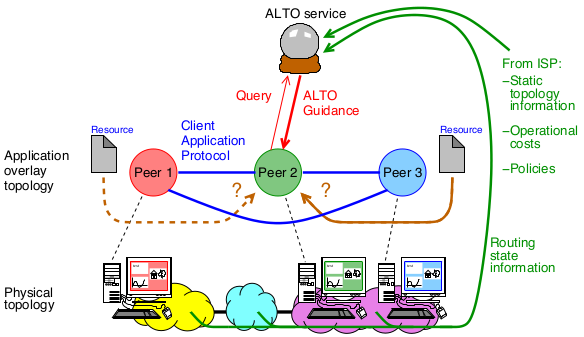
\includegraphics[scale=0.75]{alto-design.png}
    \caption{ALTO scenario of achieving traffic locality \cite{seedorf2009}}
    \label{fig:alto-design}
    \end{figure}

    Despite its origins lying in the efforts to localize traffic in \gls{p2p} applications, the \gls{alto} protocol and its encompassing system is now being considered in other fields, to be now further discussed.

    A first area of interest is \glspl{cdn}, most specifically the on-going works in extending the base protocol to implement the \gls{cdni} Request Routing Footprint \& Capabilities Advertisement interface \cite{alto-cdni}, which is a subset of the \gls{cdni} standard \cite{cdni-problem-statement} that aims to allow upstream \glspl{cdn} to query known downstream \glspl{cdn} for their willingness to accept content requests on their behalf.
    In particular, one of the main functionalities of the \gls{cdni} request routing interface is the ability for upstream \glspl{cdn} to retrieve static or dynamic information on download \glspl{cdn} (available resources, usage loads, etc.), which they provide themselves, and that allow the upstream \glspl{cdn} to better choose the appropriate edge server that could serve a given end-user.
    \gls{alto} serves as a good protocol to implement such functionality because it fits its use-case: some node wishes to improve its routing decisions to better decide on which other node to select, by using information that is hard, or nearly impossible, to independently retrieve. 
    Regarding \glspl{cdn}, the querying node is an upstream \gls{cdn} server that wishes to resolve their content requests by attributing the client to the most optimal downstream \gls{cdn} servers, where the content resides.
    At a more abstract level, this is similar to the use case already discussed, which is shown on Figure \ref{fig:alto-design}, where overlay peers required assistance to more optimally select peer connections.

    Edge computing, similarly to \glspl{cdn}, uses a paradigm of flexible service distribution that enables deployment closer to the end user for better performance, and thus is inherently effected by network status.
    Current work is being made on how \gls{alto} can be leveraged to aid the deployment of functions or applications in the network edge \cite{alto-determining-service-edge}.
    Much like the previous example, \gls{alto} is being used to guide an application in a decision that impacts both layers.
    By querying the \gls{alto} server, the client can retrieve information that regards to \gls{pop} where functions/applications can be deployed, such as cloud computing provider's available resources, e.g., \gls{cpu}, \gls{ram}, or storage, but also network information that pertains to the outside of the \gls{pop}, mainly network connectivity metrics, e.g., end-to-end bandwidth and delay, and routing costs.
    The utilization of the \gls{alto} protocol in this context would allow edge service clients and providers, as well as \glspl{isp}, the ability to combine efforts as a means to optimize edge computing deployment that considers the current network status, and doing so would thus result in benefits for both end-users and infrastructure maintainers.

    More broadly, current work is also being done in specifying \gls{ane} path arrays between points \cite{alto-path-vector} and time-specific cost values \cite{alto-calendar-cost-map}, both of which share higher insight into the network, at the discretion of the \gls{isp}, as a means to provide even more context to applications about the infrastructure, such as identifying potential path bottlenecks and times of traffic peaks, and thus improve the application's ability to optimally generate traffic.

    A mode of operation where applications no longer act in disregard of the network infrastructure they run on, but instead in deep consideration of it, could help significantly alleviate the issues emerging from the tension between the underlay and overlay, and is of mutual interest - improving application performance and reducing infrastructural costs.
    Enabling a communication channel can thus allow for many different co-operational use cases besides the aforementioned ones.
    For example, redirecting users to nearby data caches or warning them of server maintenance ahead of time.

    The existence of an all-encompassing oracle could also prove beneficial for applications which utilize periodic network probing to guide their choices, as such information could be measured by a select few nodes in the network and applicable to all nodes which are close-by in ways that the \gls{isp} deems advantageous, such as belonging to the same \gls{as} or geographically near, thus minimizing the amount of otherwise redundant probing required by all application entities that wanted some network status information.

    The oracle, besides containing measurements that could only be retrieved by the \gls{isp} itself due to its privileged access to the network, such as \gls{igp} packet inspections or secure \gls{snmp} queries, by handing over the decision-making process to the service provider entity, it is given power to better steer traffic in a way that favors internal policies and strategies, regarding, for example, peering agreements, current traffic flow of other applications, known bottlenecks, etc., that could not be deduced by the applications alone.
    Thus, in the decision of how to generate application traffic, the responsibility should reside in both the application and the infrastructure as a way to benefit all relevant parties, i.e., the end users, the application stakeholders, and the service providers.
    The \gls{alto} protocol serves as an enabler of a mutually cooperative layer interaction system that, by becoming the standard, would aid towards a sustainable life-cycle of the Internet.

    Finally, standardizing an architecture and related protocols for a clear problem domain could help a large subset of similar issues, since a well defined and tested specification would exist, thus allowing many applications to leverage the \gls{alto} protocol's functionalities to their needs, not requiring further cycles of development for a specification when one already exists.
    Also, the attempt to standardize the oracle pattern is helpful as it joins forces from many different domains which share common problems - many of which were exemplified previously - into a single specification.
    A widely accepted and used solution can evolve from a combined effort, and would target issues such as security and scalability, creating a single point of convergence that is mature enough to be adopted with confidence, accelerating the transformation of the Internet as individual players would not need to develop their own specifications.

\subsection{Architecture}

    The high-level conceptual \gls{alto} architecture can be seen in Figure \ref{fig:alto-architecture}.
        Central to the operation is the \gls{alto} server, which stores network information and provides it to querying clients.
        Such network information is provided by trustworthy and relevant entities, and could be derived by routing protocols, \gls{isp}-specific policies, historic measurements, and feedback provided by third parties regarding application performance on the network.
        Two protocols can be seen as part of the general architecture: the provisioning protocol, which is not currently contemplated by the \gls{alto} working group, should specify how information is provided to the \gls{alto} server; the \gls{alto} protocol, which is the main focus of the working group with the same name, specifies server-client interactions as a request-response interface for retrieval of network attributes.
        The \gls{alto} client is the main consumer of the \gls{alto} service, and it queries the \gls{alto} server on network information whenever it deems such data as necessary to what it's doing at a given moment, with some potential use cases discussed previously.
        An \gls{alto} client could be seen as any entity which is able to interface with the \gls{alto} protocol with the role of a client, and as such is not tied to a specific implementation - in the example of \gls{p2p} file sharing, a peer can act as an \gls{alto} client (like the example scenario in Figure \ref{fig:alto-design}), but a tracker could instead take that role, enhancing its ability of assisting peer communication by having an embedded \gls{alto} client that would then act on behalf of peers when querying for \gls{isp} insight as to provide an optimal peer pairing.
        Using the tracker-oriented \gls{alto} client approach would minimize needed \gls{p2p} client protocol modifications and thus facilitate integration with currently existing applications.

    \begin{figure}[H]
    \centering
    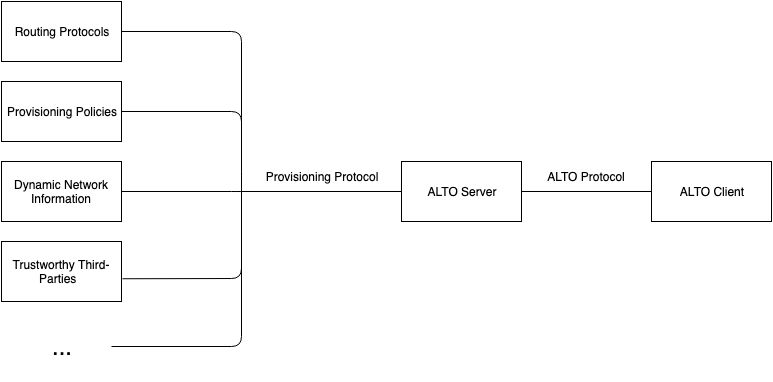
\includegraphics[scale=0.60]{alto-architecture.jpeg}
    \caption{ALTO architecture (adapted from \cite{alto-protocol})}
    \label{fig:alto-architecture}
    \end{figure}

    The \gls{alto} services contemplated by the working group can by visualized in Figure \ref{fig:alto-services}.

    \begin{figure}[H]
    \centering
    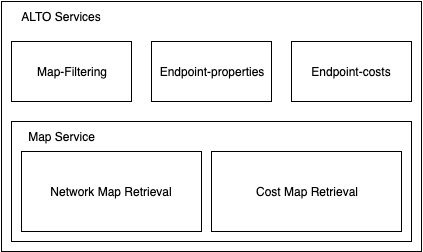
\includegraphics[scale=0.55]{alto-services.jpeg}
    \caption{ALTO services (adapted from \cite{alto-protocol}) }
    \label{fig:alto-services}
    \end{figure}

    The \gls{alto} server stores and provides special mappings in the form of network and cost maps.

    A network map provides network location grouping identifiers and the corresponding aggregated endpoints.
    It utilizes \glspl{pid} as keys, and the mapping itself is left to the responsibility of the providers.
    A provider is free to organize endpoints with the criteria he pleases, such as geographical proximity, one or many subnets, one or many \glspl{as}, etc., and attribute properties to the aggregate, instead of the endpoint.
    This is advantageous not only for scalability reasons - since it can compress information - but also because it allows \glspl{isp} to abstract network endpoints into groups, thus ensuring privacy of network topology details whilst maintaining useful network guidance, as the \gls{isp} has full control of how endpoints are aggregated, and consequentially how traffic is engineered since this changes how clients interpret resources.

    A second resource type provided is the cost map, which can be defined as a matrix M, where $M_{ij}$ - with i and j being the source and destination \glspl{pid}, respectively - is the associated path cost between the two indexes.
    The cost has two components: its metric and mode.
    The \gls{alto} base protocol only defines a single, generic, cost metric called "routingcost".
    However, \cite{alto-cost-metrics} is currently specifying more concrete metrics, with many associated with \gls{qos} evaluation, e.g., one way and round trip delay, packet loss and throughput.
    The other cost property, cost mode, can either specify that the metric is to be interpreted as a numerical value or as an ordinal ranking among all other costs in that cost map - this is useful in cases where too much network information is not deemed reasonable to share, and a simple order of preference that doesn't expose excessive infrastructural details can suffice.
    The decision to separate network and cost map information into two types of resources comes from the reasoning that network mappings are unlikely to change, whereas cost mappings could be periodically updated.
    As such, it alleviates client applications from the need to retrieve redundant information, and gives the ability to only retrieve a subset of it - this ability is further expanded in the map filtering service, which allows an \gls{alto} client to further specify which regions of the requesting maps it wishes to retrieve (much like a "SELECT" statement from an \gls{sql} database), and only these are transmitted.

    Finally, the last two services focus on mappings that regard to specific endpoints, instead of abstract mappings that utilize \glspl{pid}.
    An endpoint is currently identified by one of the following: \gls{ip} address, \gls{mac} address, or generic overlay ID.
    The endpoint property service maps to an endpoint a set of properties, e.g., geographical location or connectivity type, and the endpoint cost map has the same meaning of a cost map, but mapping to particular endpoints addresses and not abstract collections.
    The \gls{isp} has thus the ability to work with abstract aggregates or specific endpoints, showing as little or as much network information as it deems fit.

    As could be seen, the \gls{alto} project specifies an architecture for sharing of network-related information, with well defined roles and a request-response protocol to fulfill interactions between them.
    It also attempts to standardize such interactions in the form of data structures with well defined attributes which are then to be manipulated for each use case.
    This could then serve as a useful service for any application that wishes to retrieve network information as a means to improve its decision making at the application level.
    It is important to note that there are restrictions to what kinds of information are contemplated by the \gls{alto} protocol - for example, transport-level congestion is beyond its scope, and thus should not replace conventional mechanisms.
    The type of data which is valid to consider, according to the group's problem statement \cite{alto-problem-statement}, should not be easily obtainable by the clients themselves - such as immediate end-to-end delay - and should be variable on a longer timescale than the instantaneous kinds that are seen on, for example, congestion control mechanisms, as the frequently resulting querying traffic would be counterproductive to the task of traffic optimization.
    Potentially valuable information that is in the \gls{alto} scope would then have to be harder to obtain without aid of this service, and not highly mutable through time - for example, routing costs, geographical locations, network proximity, operator's policies, scheduled down-times, historical application feedback, etc.

    This project is, at time of writing, still on-working, with many drafts being created and updated as the \gls{alto} project matures and increases its domain applicability.
    These are, however, relating to service extension and deployment, since the main architecture, protocol design, implementation guidelines and security analysis are fully published into their respective \gls{rfc} documents, serving as pillars for this work, and the ongoing efforts will serve as inspirations for potential extensibility.

\subsection{Viability}

\subsubsection{Security}
\label{ssec:alto-security}

    Given the nature of this system, particularly the trading of sensitive network structure information that can alter application behavior, it is quite apparent that its design and implementation are not without challenges from a security perspective.
    Indeed, the working group published discussions regarding security preoccupations at the development and deployment stages of the \gls{alto} system \cite{alto-problem-statement} \cite{alto-protocol} \cite{alto-deployment-considerations}.

    Utilizing the "STRIDE" threat model \cite{stride}, the main threats to the \gls{alto} architecture can be summarized as follows:

\begin{itemize}
    \item Spoofing of a legitimate \gls{alto} server that would mislead clients with wrong information - this could give the malicious party the ability to change traffic to its will.
        Spoofing of the clients themselves can also occur, and could allow a malicious party to retrieve sensitive network data outside their permission.
        Finally, spoofing of a provider of network status that could feed information into the server to be spread to applications, possibly misleading them in the same way an \gls{alto} server spoofing could, but by proxy.
    \item Tampering of data to mislead either \gls{alto} servers or clients.
        If some unauthorized and malicious party can retrieve data that is in transit or storage and tampers with it, clients would act on information that they assume is trustworthy but in fact has been modified.
        As such, clients could be redirected to wrong addresses, or receive incomplete or incorrect data that results in bad decision making.
        On the other hand, data tampering that occurs between data providers and the \gls{alto} server would give the latter, from a seemingly trustworthy party, untrustworthy data.
        This would result in the same issues that could arrive from spoofing threats.
        Tampering could also occur in input forms in the server-client or server-provider interface with potential to inject malicious code execution.
    \item Repudiation of being the source of some network information, whether it be by a third party that volunteered the data or the \gls{alto} server itself, which would make it difficult to neutralize and attribute culpability to incorrect or malicious sources, jeopardizing the legitimacy of the provided network information.
    \item Information disclosure in the form of \gls{alto} resources being made available to entities that were not contemplated to access it.
            These resources could give malicious parties insight of network topology status as well as the ability to derive the client's network usage patterns by observing what kinds of resources they attempted to retrieve at a given moment.
    \item Denial of service of the \gls{alto} server through request flooding beyond its capability, which would severely hinder - or even negate - its ability to serve legitimate users.
        By proxy, service denial of external entities can also happen through the manipulation of \gls{alto} resources themselves - leveraging the system's potential to guide traffic, if a given resource is manipulated in such a way that unreasonably favors the preference of a specific subset of servers, these could be selected by clients in a disproportionate matter, and highly affect these servers' availability.
    \item Elevation of privileges that enable a user to obtain or modify more information than initially permitted, resulting in the previous threats being heightened.
\end{itemize}

    Many of these threats are standard preoccupations for most computing systems and could be solved with state of the art solutions which are well proven and tested, as indeed states \cite{alto-protocol}.
    However, regarding threats of information disclosure, whilst they can be negated with in-transit encryption, what is done with this information the moment it reaches the client is hard to control - situations may arise when a client with proper resource permissions shares, intentionally or not, sensitive network information with other users who may or may not have proper clearance, in interactions outside the \gls{alto} architecture.
    Furthermore, many authenticated clients with different permissions could share information, which they retrieved legitimately, among themselves, to get an illegitimate complete view of the network structure.
    Thus, individual clients could internally collaborate outside the system to bypass access control measures applied inside it.
    As such, it is firstly important for the \gls{isp} or third parties to carefully plan on what information they are comfortable with sharing, knowing that it may be susceptible to future disclosure outside the secure domain.
    Possible solutions to minimize these threats include:

\begin{itemize}
    \item Reduce the granularity of the provided data.
        Intuitively, the less granular and precise the shared information by the \gls{alto} server is, the less valuable the resulting application guidance will be, and thus a balance would have to be found between layer cooperation and \gls{isp} privacy.
        One example is the usage of network groupings by \glspl{pid} instead of mapping information to concrete endpoints, working with network status about abstract entities.
        Another possible mean to reduce information granularity would be to utilize ordinal cost values, which instead of specifying a concrete metric, e.g., bandwidth in bits per second or packet loss in percentages, the server would give a relative preference rating with lower costs meaning lower preference.
        In both examples, the granularity of network information transmitted to the client is several levels higher in abstraction than the actual physical layer, and this could reduce the flexibility of applications to optimize traffic.
        However, the oracle service can still provide acceptable flexibility without considerably impacting \gls{isp} privacy, acting as a much needed compromise.

    \item Work only with a small set of trustworthy \gls{alto} clients that are to act on behalf of a larger subset of less trustworthy clients.
        For example, network status resources could only be provided to authorized cooperation-oriented trackers in the BitTorrent protocol, which would in turn use this information to provide customized replies to clients without the need to change the base protocol.
        Similarly, information relevant for user-server assignment could only be provided to authenticated \gls{cdn} control nodes, who'd use among themselves a private virtual domain to share information about user-server connectivity and server status that would otherwise be inappropriate for any other type of user to retrieve.
        This is still, however, worthy of further threat analysis as restricted information could still leak outside of the system - beyond the means of spoofing discussed previously, seeing how a system behaves with \gls{alto} guidance can give - albeit limited - insight into \gls{ISP} bias.
        To see this, consider how a BitTorrent peer could continuously query a tracker with carefully crafted parameters - such as source address and candidate peers - and attempt to derive information from the resulting action, or similarly how a end-user could utilize similar parameter modifications to observe the edge server selection mechanism in action.

    \item Utilize terms of agreement that are to be enforced on every querying client, stating that network status information does not get used beyond its original purpose, prohibiting sharing.
        Although a potentially helpful mechanism to dissuade malicious users, it can be deemed impractical to apply, especially considering the scale at which this information could be shared.
        Thus, such means should be applied at a case-by-case situation and it should not replace \gls{isp} discretion and server resource maintenance to ensure a given standard.
\end{itemize}

<BOOKMARK 18/01/21>

\subsubsection{Privacy}%

    Privacy concerns are also very prevalent in the \gls{alto} system, being an ubiquitous talking point in most of the working group's problem statements and protocol specifications.
    When an \gls{alto} client queries a server for one or more network status resources in the attempt to optimize the application traffic it will generate in the near future, certain parameters can be passed to the server that can make the response be more personalized and contain more granular information.
    For example, a real-time \gls{p2p} media-streaming application seeking \gls{alto} guidance to help choose among a list of candidate streaming peers may wish to include in its query helpful parameters such as the peer list itself, the desired \gls{qos}, and the network position of the querying client itself.
    Indeed, these and more patterns will help increase the effectiveness of the \gls{alto} server's guidance in helping the client application achieve its goal, but such happens at the expense of potentially allowing an \gls{alto} server to infer on user pattern statistics.
    Even assuming that the previously discussed information disclosure threats are nonexistent in the \gls{alto} system, privacy concerns can arrive from client applications because the resource queries they need to produce can contain information about what the client either will or wants to do.
    This is recognized by the \gls{alto} working group as a possible concern \cite{alto-protocol} \cite{alto-problem-statement}.
    In response, they state that the clients should firstly be cognizant about the potential tracking risk that is associated with the usage of the system and, as an attempt to make tracking harder, they could disable \gls{http} cookies and/or opt for more vague query parameters, e.g. by randomizing some bits on endpoint addresses or simply using more broad addresses, whilst being aware that the helpfulness of query results may vary with increased parameter obfuscation.

    Very much like client privacy, \gls{isp}-related privacy is also considered by the working group.
    \glspl{pid} were created as a means for \glspl{isp} to abstract network components as a collection of single network endpoints with similar properties, helping them not to disseminate network information that is too sensitive, and in turn also allows clients to make queries based on these identifiers and maintain a higher level of privacy.
    An ongoing proposal for protocol extension includes path vectors \cite{alto-path-vector}, that aim to represent information on the intermediary hops from a given source-destination pair, and each of these hops is represented as an \gls{ane} that, similar to \glspl{pid}, give \glspl{isp} the ability to under or over-abstract the topological representation that gets published to clients, giving more options to balance guidance usefulness with provider privacy.
    Other solutions could also be considered depending on the needs of the clients and the direction of the project as a whole.
    For example, the servers themselves could operate on a secure communications channel and maintain a clear agreement on what can and cannot be made with the collected information.
    Alternatively, clients that wish not to impose much trust on the server's claims not to track them could make bulk queries (or use proxies to do so for them) and privately filter out the relevant information, heavily restricting on the ability to retrieve user activity patterns.

\subsubsection{Incentivisation}

    Incentivization relates to creating and divulging, to both layers, incentives to a fully cooperative layer relationship that is inherent in the oracle pattern adopted by the \gls{alto} system.
    It is quite the challenge to fundamentally change how applications behave on the Internet, as indeed is to ask of \glspl{isp} to launch a view of their infrastructure to the outside world.
    \cite{dan-Commag10} notes incentivisation as one of the key challenges in overlay-underlay cooperation in regards to \gls{p2p} applications, stating that incentive mechanisms need to exist to ensure that both layers agree to participate in, and maintain, a cooperative relationship.
    According to the \gls{alto} problem statement \cite{alto-problem-statement}, the incentives for both parties to act on the system are the advantages that derive from using it.
    Meaning, clients are to expect better application performance by leveraging \gls{alto} guidance, and similarly \glspl{isp} should expect that their internal goals, such as an optimization of infrastructure utilization, can be met with the increased traffic engineering ability that results from their oracle role.
    If the overlay consuming \gls{alto} guidance has a manageable number of accountable entities, such as a single \gls{cdn} or data center that the \gls{isp} agrees to partner with, it is realistic to maintain a cooperative agreement that can be solidified with feedback and service agreements.
    However, if the overlay utilizing the \gls{alto} system makes it hard to pinpoint accountability, such as a large \gls{p2p} application with many users, it will naturally be harder to ensure that the power dynamic between layers doesn't shift beyond an equilibrium.
    In these cases, policies could be created and enforced to give insurance to both parties that a cooperative relationship is maintained.

    The \glspl{isp} could too, like mentioned above, lack proper cooperation, as they are found in a new power dynamic that would leverage their application traffic engineering capabilities to steer traffic in a way that is advantageous to only them, or at least in a disproportionate manner.
    Again, much like the lack of cooperation by clients, it is difficult to guarantee an equilibrium in the power dynamic between layers, but by guaranteeing improved \gls{qos} levels for applications that utilize \gls{alto} cooperation, \glspl{isp} become responsible for guaranteeing that these improvements are met, fearing client abandonment otherwise.
    Giving freedom to both layers on how they act ensures that the system evolves to a common ground that benefits both sides, at least enough to justify them remaining there.

    Finally, if the application-\gls{isp} tussle becomes harsher and unmaintainable, which is a point that was argued for in the network infrastructure effects portion in Section \ref{sec:state-of-art}, a cooperative system such as \gls{alto} may become necessary, and thus beyond preferable, meaning that \glspl{isp} may be forced to block or throttle traffic that it cannot route properly, as it historically happened.
    Thus, acting with \gls{alto} could go beyond a voluntary action into a symbiotic necessity, meaning that both parties have to act cooperatively to maintain network sustainability.
    Regardless, the best approach seems to be that the system must in of itself be self-justifiable, meaning that the advantages that it brings should be enough to convince both parties to act on it.
    \glspl{isp} are nevertheless free to deploy their own incentive mechanisms to facilitate early application adoption, that could include monetary rewards or routing privileges, but doing so could damage network neutrality.

\subsubsection{Network Neutrality}
    As stated by \cite{qos-framework}: "According to most network neutrality proponents, network neutrality rules are intended to preserve the Internet's ability to serve as an open, general-purpose infrastructure that provides value to society over time in various economic and non-economic ways. In particular, network neutrality rules aim to foster innovation in applications, protect users' ability to choose how they want to use the network, without interference from network providers, and preserve the Internet's ability to improve democratic discourse, facilitate political organization and action and to provide a decentralized environment for social, cultural and political interaction in which anyone can participate.".
    Network neutrality has been a popular point of discussion as society grows around the Internet, sparking debates around the world on what the best course of action should be - for example, regulations were introduced by the \gls{fcc} \cite{fcc} in the United States to police network neutrality \cite{fcc}, and the European Union has a framework for net neutrality laid down in Article 3 \cite{article-3}.
    However, potential violators of the spirit of a network neutrality exist, such as British Plusnet's \cite{plusnet} usage of \gls{dpi} to implement limits and differential charges for different traffic \cite{arstechnica}, or Portuguese MEO's \cite{meo} smartphone contracts which include zero rating programs for a given set of services \cite{meo-packages} that bundle applications such as Facebook \cite{Facebook} or Spotify \cite{spotify}.

    Network neutrality advocates are concerned with guaranteeing that \glspl{isp} keep Internet communications free and do not discriminate based on the traffic's specifics, such as platforms, applications, or source and destination addresses.
    On the other hand, opponents of net neutrality, among them the \glspl{isp} themselves, broadband and telecom companies, and hardware manufactures, argue against net neutrality - they claim that it would would reduce incentive to invest, as investments would be harder to insure without the ability to charge higher rates for better infrastructure capabilities.
    Zero rating programs, such as Wikipedia Zero \cite{wikipedia-zero}, which provide Wikipedia \cite{wikipedia} pages with no charge to a select group of low income regions, are popular in developing countries \cite{network-neutrality-developing} , provide to select regions Internet content they could not otherwise get, but in the form of a non-neutral view to the network.
    Additionally, with net neutrality, the \gls{isp}'s ability to route traffic could itself be at jeopardy - as \cite{qos-aware} states when he argues for a solution that compromises net neutrality via service differentiation, the Internet is growing at an astonishing rate, as are the demands of applications, and operating the infrastructure on a purely best-effort basis will not be sufficient without a constant provisioning of such infrastructure to keep up with demand, and this too may not be economically viable nor even possible.
    Thus, discriminating by traffic services may be needed to guarantee that, say, real-time medical information gets priority over real-time media streaming, which in turn gets priority over e-mail or file sharing.

    Considering that the \gls{alto} system behaves in an oracle pattern of cooperation where a single entity - the \gls{isp} - is able to heavily influence the traffic patterns of the applications it aids, on the promise of a cooperative network underlay-overlay relationship, such system could violate the principles of net neutrality.
    In particular, this could happen if the oracle either blocks, or at the very least provides different guidance to different clients, depending on where the query originated from - e.g., which application, which source address, or other defining characteristics.
    A possible consequence of such a system guiding the Internet could be that given applications can consistently have better \gls{qos} measurements not on the basis of the application's implementation, but on the \gls{isp} personal biases.
    Oracle systems such as \gls{alto} do not seem to be analogous to other traffic engineering strategies, such as the usage of \gls{mpls}, \gls{diffserv}, nor to other means of \gls{isp} intervention on overlays, such as the deployment of data caches and redirector proxies - this is because the oracle system, in contrast to the previously mentioned strategies, is one of mutual voluntary and cooperative nature between \glspl{isp} and applications.
    However, it could be argued that if the \gls{alto} system offered guidance to applications in such a way that consistently resulted in better application performance, such applications would be pressured to use such guidance as a means to remain competitively viable, and the \glspl{isp} would then have a platform to influence a considerable amount of traffic to their will, being in a position to, depending on how they treat guidance requests, break network neutrality.
    This neutrality concern can be alleviated if application guidance operated on classes of traffic, e.g. real-time communication or file sharing, thus operating on traffic aggregates to insure \gls{qos} levels needed to given application types, but never discriminating beyond such given classes.

    As the protocol is defined \cite{alto-protocol}, the provided network status information is truthful and guidance is optional, and neutrality can then still remain outside of the system, since no routing measurements exist within it.
    If particular implementations of the \gls{alto} system give guidance in such a way to guide traffic in a discriminatory fashion, and if such guidance has advantages that much outweigh any alternative, thus rendering it beyond optional,  a case can be made for how \gls{alto} as a concept can break network neutrality, considering all its advantages and disadvantages discussed below, as the \gls{isp} can utilize discriminatory behaviour to treat applications on their infrastructure differently.

\subsubsection{Multi-Domain orchestration}

    The Internet as we know it today spans the entire globe and is rather complex in nature.
    According to \cite{dan-Commag10}, the classic vision of the Internet consisting of a network of transit and stub \glspl{as} no longer seems accurate, as it now is much more complex - for starters, the role of network owner and service provider are separating, and Internet access is provided by numerous competing \glspl{isp}.
    As a demonstration of such complexity, Figure \ref{fig:network-connectivity-globe} displays how the Internet is structured into many tiers of different service providers.

    Considering this administrative complexity in the Internet's topology, it can thus be inferred that the act of layer cooperation can get harder when the influence domain increases and potentially spans many different \gls{isp} regions which will inevitably act differently as they can have different technologies, biases, policies, and overall goals.
    These per-\gls{isp} biases can make it difficult to guarantee that traffic optimization spanning multiple administrative domains is actually useful and achieves the cooperative nature in mind.
    For example, an \gls{isp} may not be comfortable categorising end-point costs of a given metric, thus making path calculations that pass through that \gls{isp} domain not viable.
    Regardless, per-domain \gls{isp} guidance has nonetheless plenty of potential, e.g., the ability to localize traffic, as entities outside of domain can be identified by \gls{isp}, and similarly per-domain optimization of resources can still be useful when such domain is large, and can be applied to high-volume operations such as those in a data center.
    The \gls{alto} server within a given domain can also leverage probing measurements and feedback statistics to derive information in areas whose topological detail is unknown, giving a partial network view that contains topological insight and also information derivation that, whilst not being as good as a complete topological insight, may nonetheless power a cooperative effort within a given domain with good results.
    Some data may, whoever, be both not shared by an external domain nor derivable.
    This includes endpoint property information, such as network connection types, or server footprints, e.g., available \gls{cpu}, \gls{ram} and storage.
    This information can in some conditions only be retrieved by authoritative entities in a given domain and probing solutions may not be available, thus considerably limiting the applicability of a single \gls{alto} domain.

    \begin{figure}[H]
    \centering
    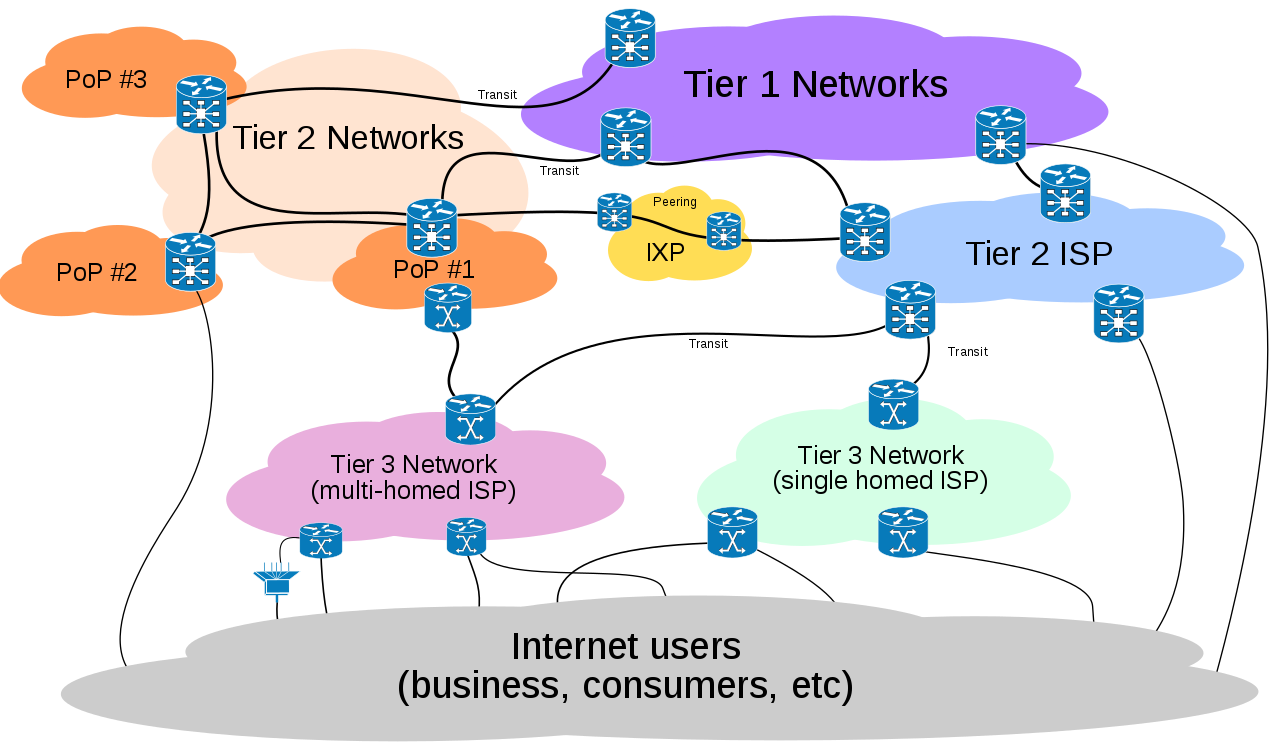
\includegraphics[scale=0.30]{network-connectivity-globe.png}
    \caption{Conceptual representation of ISP diversity on the Internet}
    \label{fig:network-connectivity-globe}
    \end{figure}

    Even assuming that all \glspl{isp} are comfortable with sharing sufficient information, ambiguity may arise.
    For example, considering a cost map with the generic "routingcost" cost metric, \glspl{isp} could internally calculate routing costs differently, and prioritizing different goals, e.g., reducing overall link usage versus reducing inter-\gls{as} traffic first and foremost.
    The base \gls{alto} protocol specification states that each network region can provide its \gls{alto} services, which in turn convey network information from their perspective.
    A network region, per the protocol specification, consists of a given administrative domain, such as an \gls{as}, an \gls{isp}, or a given set of agreeing \glspl{isp} \cite{alto-protocol}, thus implying that if multiple \glspl{isp} share an \gls{alto} server they must reach a consensus on what network status is available for query from the outside.
    Furthermost, the \gls{alto} working group's deployment considerations \cite{alto-deployment-considerations} document states that an \gls{alto} client can query a single server for one or many metrics, or he can additionally query multiple server instances on different networks \cite{alto-deployment-considerations}.
    It is explicitly stated in the document that each server could give guidance for only a given network partition, and such guidance may wildly differ between them due to the fact that different algorithms and objectives may have been applied.
    The document also states that, in regards to extending the reachability of a single server, three different strategies could be applied:

\begin{itemize}
    \item \textbf{Authoritative Servers}: A given set of servers can provide guidance for all kinds of destinations to all \gls{alto} clients.
    \item \textbf{Cascaded Servers}: An \gls{alto} server can possess an embedded \gls{alto} client and query other neighbouring servers if it cannot serve the original request, acting as a middleman between the client and the more appropriate servers.
    \item \textbf{Inter-server Synchronization}: Different \gls{alto} servers communicate among themselves to expand the knowledge space.
\end{itemize}

    The last strategy is still being subject to development and standardization by the working group as part of a bigger attempt to link different network regions and technologies into a single, homogeneous abstraction of the Internet.
    Current efforts in multi domain orchestration and relevant use case examples are summarized in the ongoing work of \cite{alto-multi-domain-use-cases}.

\section{Summary}

    In the taken case studies seen in this chapter, it can be clearly seen that there is room for improvement in application-layer traffic generation that can benefit both the applications themselves and the infrastructure administrators that support them.
    Applications struggle to achieve optimal network resource utilization, whether that be in the task of matching peers in overlay networks, deploying and attributing edge server to media clients, selecting mirror servers, etc., and solutions are being continuously proposed and created that attempt to optimize these decisions.
    Traffic optimization solutions vary between them with the range of control that is given to the overlay and underlay parties.
    It seems to be the case that one-sided solutions can hurt the other layer in a worse case scenario, and be lacking maximum efficiency at the best.
    \gls{alto}'s proposal seems to bridge the best of both types of proposals that are either underlay or overlay-centric, standardizing a system and associated protocol whose purpose is to achieve layer cooperation so proper network utilization is possible.
    Despite many of its associated challenges - namely in the regions of security, privacy, and incentivisation - the project certainly has the potential for a more resourceful Internet that can be more sustainable.
